\documentclass[11pt,a4paper]{report}

% ---------- Encoding & Language ----------
\usepackage[utf8]{inputenc}
\usepackage[T1]{fontenc}
\usepackage[english]{babel}

% ---------- Typography ----------
\usepackage{mathptmx}            % Times-like serif body
\usepackage[scaled=0.9]{helvet}  % Helvetica-like sans for headings
\usepackage{courier}             % Monospace
\usepackage{microtype}
\usepackage{setspace}
\onehalfspacing

% ---------- Page Geometry ----------
\usepackage[a4paper,top=2.5cm,bottom=2.5cm,left=2.8cm,right=2.5cm,headheight=14pt]{geometry}

% ---------- Colors ----------
\usepackage[dvipsnames,table]{xcolor}
\definecolor{PrimaryBlue}{RGB}{28,64,122}
\definecolor{AccentBlue}{RGB}{70,130,180}
\definecolor{SoftGray}{RGB}{240,240,240}
\definecolor{RuleGray}{RGB}{170,170,170}
\definecolor{CodeBg}{RGB}{246,246,246}
\definecolor{CodeBorder}{RGB}{220,220,220}
\definecolor{CodeKey}{RGB}{30,90,160}
\definecolor{CodeStr}{RGB}{160,40,40}
\definecolor{CodeCom}{RGB}{90,110,90}

% ---------- Headings ----------
\usepackage{titlesec}
\titleformat{\chapter}[display]
  {\normalfont\sffamily\Huge\bfseries\color{PrimaryBlue}}
  {\filleft\Large Chapter \thechapter}
  {1ex}
  {\titlerule[1pt]\vspace{1ex}\filright}
  [\vspace{-0.5ex}{\color{RuleGray}\titlerule[0.5pt]}]
\titlespacing*{\chapter}{0pt}{-20pt}{24pt}

\titleformat{\section}
  {\normalfont\sffamily\Large\bfseries\color{PrimaryBlue}}
  {\thesection}{0.75em}{}
\titleformat{\subsection}
  {\normalfont\sffamily\large\bfseries\color{AccentBlue}}
  {\thesubsection}{0.6em}{}
\titleformat{\subsubsection}
  {\normalfont\sffamily\normalsize\bfseries}
  {\thesubsubsection}{0.5em}{}
\titleformat{\paragraph}[runin]
  {\normalfont\sffamily\normalsize\bfseries}
  {}{0em}{}[.]

\titlespacing*{\section}{0pt}{18pt}{8pt}
\titlespacing*{\subsection}{0pt}{14pt}{6pt}
\titlespacing*{\subsubsection}{0pt}{10pt}{4pt}

% ---------- Headers & Footers ----------
\usepackage{fancyhdr}
\pagestyle{fancy}
\fancyhf{}
\renewcommand{\chaptermark}[1]{\markboth{\thechapter.\ #1}{}}
\renewcommand{\sectionmark}[1]{\markright{\thesection.\ #1}{}}
\fancyhead[R]{\small\sffamily\thepage}
\fancyhead[L]{\small\sffamily\nouppercase{\leftmark}}
\renewcommand{\headrulewidth}{0.4pt}
\renewcommand{\headrule}{\color{RuleGray}\hrule width\headwidth height\headrulewidth}

\fancypagestyle{plain}{%
  \fancyhf{}%
  \fancyfoot[C]{\small\sffamily\thepage}%
  \renewcommand{\headrulewidth}{0pt}%
}

% ---------- Tables ----------
\usepackage{booktabs}
\usepackage{longtable}
\usepackage{tabularx}
\usepackage{array}
\renewcommand{\arraystretch}{1.25}
\newcolumntype{L}[1]{>{\raggedright\arraybackslash}p{#1}}
\newcolumntype{C}[1]{>{\centering\arraybackslash}p{#1}}

% ---------- TikZ / Diagrams ----------
\usepackage{tikz}
\usetikzlibrary{positioning,arrows,shapes.geometric,fit,backgrounds,calc}
% Define color palette for architecture diagrams
\definecolor{LayerClient}{RGB}{232,241,252}
\definecolor{LayerAPI}{RGB}{224,238,247}
\definecolor{LayerOrch}{RGB}{215,232,244}
\definecolor{LayerAgents}{RGB}{204,228,241}
\definecolor{LayerTools}{RGB}{194,224,239}
\definecolor{LayerData}{RGB}{183,218,234}
\definecolor{BoxBorder}{RGB}{70,130,180}
\definecolor{BoxFill}{RGB}{255,255,255}
\definecolor{Accent}{RGB}{28,64,122}

% ---------- Lists ----------
\usepackage{enumitem}
\setlist{itemsep=3pt,parsep=0pt,topsep=4pt}

% ---------- Graphics ----------
\usepackage{graphicx}
\usepackage{float}
\graphicspath{{figures/}}

% ---------- Code listings ----------
\usepackage{listings}
\lstdefinelanguage{TypeScript}{
  keywords={var,let,const,function,return,import,export,from,new,async,await,if,else,while,for,case,switch,break,default,extends,class,interface,type,enum,public,private,protected,readonly,static,this,true,false,null,undefined,as,in,of,typeof,instanceof,throw,try,catch,finally},
  keywordstyle=\color{CodeKey}\bfseries,
  ndkeywords={string,number,boolean,any,void,Promise,BaseChatModel,ReadableStream,Response},
  ndkeywordstyle=\color{CodeKey!70!black},
  identifierstyle=\color{black},
  sensitive=true,
  comment=[l]{//},
  morecomment=[s]{/*}{*/},
  commentstyle=\color{CodeCom}\itshape,
  stringstyle=\color{CodeStr},
  string=[b]',
  morestring=[b]",
}
\lstset{
  basicstyle=\ttfamily\footnotesize,
  backgroundcolor=\color{CodeBg},
  rulecolor=\color{CodeBorder},
  frame=single,
  framesep=6pt,
  breaklines=true,
  breakatwhitespace=true,
  columns=fullflexible,
  tabsize=2,
  showstringspaces=false,
  captionpos=b,
  aboveskip=10pt,
  belowskip=10pt,
  xleftmargin=4pt,
  xrightmargin=4pt,
}
\lstdefinestyle{tsstyle}{language=TypeScript}
\lstdefinestyle{shstyle}{language=bash,keywordstyle=\color{CodeKey}\bfseries,basicstyle=\ttfamily\footnotesize}
\lstdefinestyle{jsonstyle}{
  basicstyle=\ttfamily\footnotesize,
  keywordstyle=\color{CodeKey}\bfseries,
  stringstyle=\color{CodeStr},
  commentstyle=\color{CodeCom}\itshape,
  morekeywords={true,false,null},
  morestring=[b]",
  morecomment=[l]{//},
}

% ---------- Quotation and inline code ----------
\usepackage{csquotes}
\usepackage{xurl} % allow URL line breaking at any character
\newcommand{\code}[1]{\texttt{\small #1}}

% ---------- Hyperlinks & PDF metadata ----------
\usepackage[pdfusetitle,colorlinks=true,linkcolor=PrimaryBlue,urlcolor=AccentBlue,citecolor=PrimaryBlue,bookmarksnumbered=true]{hyperref}
\usepackage{bookmark}

% ---------- Title info ----------
\title{\Huge\sffamily\bfseries Multi-Agent AI Framework\\[0.4em]
\LARGE\mdseries Final Project Report}
\author{\sffamily DeepStackers Team}
\date{\sffamily April 2026}

% Allow TeX to stretch paragraph lines by a small amount before overflowing.
\emergencystretch=3em
\hbadness=10000
\hfuzz=2pt

\begin{document}

% =====================================================================
% Title page
% =====================================================================
\begin{titlepage}
  \centering
  \vspace*{2cm}
  {\color{RuleGray}\rule{\linewidth}{0.8pt}}\\[1.5em]
  {\sffamily\Huge\bfseries\color{PrimaryBlue} Multi-Agent AI Framework}\\[1.5em]
  {\sffamily\LARGE\bfseries\color{PrimaryBlue} for Task-Aware Model Routing}\\[1.5em]
  {\sffamily\LARGE\bfseries\color{PrimaryBlue} and Execution}\\[1.5em]
  {\color{RuleGray}\rule{\linewidth}{0.8pt}}\\[1.5em]

  {\sffamily\Large\bfseries Final Project Report}\\[2.5em]

  {\sffamily\large\bfseries\color{PrimaryBlue} Team DeepStackers}\\[1.2em]

  {\sffamily\large Oruç Çakır}\\[0.35em]
  {\sffamily\large Mehmet Gür}\\[0.35em]
  {\sffamily\large Serin Evcim}\\[0.35em]
  {\sffamily\large Ömer İlbilgi}\\[0.35em]
  {\sffamily\large Ulaş Kaya}\\[2em]

  {\sffamily\normalsize April 2026}
\end{titlepage}

% =====================================================================
% Table of contents
% =====================================================================
\pagenumbering{roman}
\setcounter{tocdepth}{2}
\tableofcontents
\clearpage

% =====================================================================
% Abstract
% =====================================================================
\chapter*{Abstract}
\addcontentsline{toc}{chapter}{Abstract}
\thispagestyle{plain}
The \textbf{Multi-Agent AI Framework} is a production-ready, enterprise-grade
system designed for intelligent task orchestration across specialized AI
agents. It implements a plugin-based architecture in which individual agents
handle domain-specific operations while a centralized \emph{MainAgent} routes
user requests to the appropriate specialist. The system leverages LangGraph
for stateful computation, supports twelve LLM providers, and delivers
real-time streaming execution with persistent state management. This report
documents the final architecture, the new tools and technologies adopted, the
engineering, economic, environmental, and societal impact of the solution, a
survey of relevant prior work and engineering principles, and a comprehensive
test evaluation of the delivered system.

\clearpage
\pagenumbering{arabic}

% =====================================================================
% CHAPTER 1 — Final Status and System Architecture
% =====================================================================
\chapter{Final Status and System Architecture}

\section{Final System Architecture and Design}

\subsection{Executive Summary}

The Multi-Agent AI Framework is a production-ready, enterprise-grade system
designed for intelligent task orchestration across specialized AI agents. It
implements a sophisticated plugin-based architecture where individual agents
handle domain-specific operations while a centralized MainAgent intelligently
routes user requests to the appropriate specialist. The system leverages
LangGraph for stateful computation, supports twelve LLM providers, and
provides real-time streaming execution with persistent state management.

\subsection{Core Architectural Principles}

\subsubsection{Self-Registration Pattern}

The framework employs a \textbf{self-registration pattern} where each
specialized agent registers itself at module load time with the central
\code{AgentRegistry}. This decoupled approach eliminates tight coupling
between agents and the MainAgent:

\begin{itemize}
  \item Each agent module instantiates itself and automatically registers with \code{agent\-Registry.\allowbreak register()}.
  \item The registry maintains metadata: unique ID, human-readable name, delegation tool name, tool description, and task prefix.
  \item MainAgent dynamically discovers registered agents and builds its orchestration graph accordingly.
  \item New agents can be added without modifying MainAgent or the registry implementation.
\end{itemize}

\begin{lstlisting}[style=tsstyle,caption={Each agent self-registers at module load time.}]
// Pattern Example: each agent self-registers
export const githubAgent = new GitHubAgent(GitHubAgentConfig, tools);

agentRegistry.register({
  id: githubAgent.id,
  name: githubAgent.name,
  toolName: "delegate_to_github",
  toolDescription: "Route the task to the GitHub Agent...",
  taskPrefix: "[GitHub Task]",
  instance: githubAgent,
  getCompiledGraph: () => githubAgent.getCompiledGraph(),
});
\end{lstlisting}

\subsubsection{BaseAgent Abstraction Framework}

All specialized agents inherit from \code{BaseAgent<T extends AgentImplMetadata>},
a comprehensive abstract class that encapsulates:

\begin{itemize}
  \item \textbf{LLM Factory Integration:} dynamic LLM creation supporting twelve providers, each with provider-specific configuration and initialization.
  \item \textbf{LangGraph State Management:} automatic construction of state graphs with a standardized node structure (\code{agentNode} $\rightarrow$ \code{tools} $\rightarrow$ routing).
  \item \textbf{Tool Binding:} declarative tool binding to LLM instances with automatic tool-schema validation.
  \item \textbf{Streaming Pipeline:} structured JSON event streaming with lifecycle events (\code{AGENT\_STARTED}, \code{TOOL\_STARTED}, \code{AGENT\_STREAM}, \code{TOOL\_ENDED}, \code{AGENT\_ENDED}).
  \item \textbf{Runtime Configuration:} support for user-specific LLM overrides and secret management with configuration-version caching.
  \item \textbf{Error Handling:} graceful degradation with fallback messages and comprehensive error logging.
\end{itemize}

The BaseAgent handles the mechanical aspects of agent orchestration, allowing
specialized agents to focus purely on domain logic through tool
implementations.

\subsubsection{LangGraph StatefulGraph Architecture}

The framework uses LangGraph's \code{StateGraph} pattern with
\code{MessagesAnnotation} as the canonical state representation:

\begin{center}
\code{State = \{ messages: BaseMessage[] \}}
\end{center}

\textbf{Node structure:}

\begin{description}[leftmargin=1.6em,style=nextline]
  \item[I. Agent Node (processor).]
    \textit{Input:} current message state.
    \textit{Operation:} system-instruction prepending and LLM invocation with tool binding.
    \textit{Output:} \code{AIMessage} with \code{tool\_calls}.
  \item[II. Logic Router (decision bridge).]
    If \code{last\_message} contains \code{tool\_calls} $\rightarrow$ Tools Node; otherwise $\rightarrow$ END.
  \item[III. Tools Node (execution).]
    Concurrent execution of requested tools, conversion of raw tool outputs into \code{ToolMessages}, and cyclic transition back to the Agent Node.
\end{description}

\subsection{Multi-Agent Orchestration System}

\subsubsection{MainAgent Orchestrator Architecture}

The MainAgent implements an intelligent routing system that determines
whether to answer directly or delegate to a specialized agent:

\begin{enumerate}
  \item \textbf{Initialization phase.}
  \begin{itemize}
    \item Imports all specialized agent modules (triggering self-registration).
    \item Queries \code{AgentRegistry} for all available agents.
    \item Dynamically builds the orchestration graph with one node per agent.
  \end{itemize}
  \item \textbf{Task routing flow.} User input is sent to the MainAgent LLM (with delegation tools bound). If a delegation tool is called, the target agent is identified from the registry, routed to a \code{Prepare\_\{agent\_id\}\_Task} node, its task prefix injected (e.g.\ ``\code{[GitHub Task]}''), and the agent's compiled graph is executed. The result is returned to the MainAgent for summarization. If no delegation occurs, the answer is returned directly to the user.
  \item \textbf{Dynamic graph construction.} For each registered agent the orchestration graph adds a \code{Prepare\_\{agent\_id\}\_Task} node (that extracts the task from the delegation tool call and prepends the agent-specific prefix), an \code{\{agent\_id\}\_Subgraph} node that references the agent's compiled graph, and edges wiring MainAgent $\rightarrow$ Prepare $\rightarrow$ Subgraph $\rightarrow$ MainAgent.
\end{enumerate}

\subsubsection{Main Agent and Specialized Agent Interaction}

The delegation mechanism employs a hand-off protocol:

\begin{itemize}
  \item \textbf{Delegation tool creation:} for each registered agent, MainAgent creates a dynamic tool (e.g.\ \code{delegate\_to\_github}, \code{delegate\_to\_codebase}) using the agent's metadata.
  \item \textbf{Task extraction:} the Prepare node extracts the task description from the tool-call arguments.
  \item \textbf{Task prefix injection:} the agent-specific prefix is prepended to guide the agent's system prompt context.
  \item \textbf{Subgraph execution:} the agent's complete graph runs as a node within the MainAgent's graph.
  \item \textbf{Result integration:} agent output is automatically captured and passed back to MainAgent for synthesis.
\end{itemize}

\subsubsection{Configuration Cascading System}

The framework supports runtime configuration overrides with intelligent caching:

\begin{enumerate}
  \item \textbf{Default configuration.} Each agent has statically defined implementation metadata (provider, model, system instruction).
  \item \textbf{Runtime configuration override.} Users can specify runtime preferences that override defaults:
\begin{lstlisting}[style=tsstyle]
runtimeConfig: {
  provider: "openai",
  modelID: "gpt-4-turbo",
  subAgentConfigs: {
    "codebase": { modelID: "gpt-4-mini" }   // Override specific agent
  }
}
\end{lstlisting}
  \item \textbf{Configuration version tracking.} Each configuration change is assigned a unique version string; cached graphs are reused if the version has not changed; unnecessary LLM and tool recreation is avoided.
\end{enumerate}

\subsection{Specialized Agent Implementations}

\subsubsection{GitHub Agent}
\begin{itemize}
  \item \textbf{Tools:} 19 MCP-wrapped tools (\code{list\_commits}, \code{create\_branch}, \code{search\_code}, \dots).
  \item \textbf{Integration:} \code{StreamableHTTPClientTransport} for GitHub Copilot MCP server.
  \item \textbf{Authentication:} \code{GITHUB\_PAT} environment variable.
  \item \textbf{Capabilities:} full GitHub API operations (commits, PRs, issues, branches, code search, file operations).
\end{itemize}

\subsubsection{Codebase Agent}
\begin{itemize}
  \item \textbf{Tools:} semantic code search via pgvector embeddings.
  \item \textbf{RAG pipeline:} TypeScript/Python parsing, chunking by function / class / method.
  \item \textbf{Embedding model:} Google \code{text-embedding-004} (768-dimensional vectors).
  \item \textbf{Search:} cosine similarity with HNSW index, top-$k$ snippet retrieval.
  \item \textbf{Indexing:} offline process (\code{pnpm index:codebase}) with pgvector storage.
\end{itemize}

\subsubsection{Google Workspace Agent}
\begin{itemize}
  \item \textbf{Services:} Gmail, Google Drive, Google Docs, Google Sheets, Google Slides, Google Calendar.
  \item \textbf{Authentication:} OAuth2 with Google Auth flow.
  \item \textbf{Tools:} 27 tools across 6 services (Gmail: 6, Calendar: 5, Drive: 7, Docs: 3, Sheets: 4, Slides: 2).
  \item \textbf{Email safety:} confirmation dialog before sending (dry-run support).
\end{itemize}

\subsubsection{Search Agent}
\begin{itemize}
  \item \textbf{Tools:} 9 tools for comprehensive web research.
  \item \textbf{Search engines:} DuckDuckGo (web, news, images), Exa API (semantic search, academic research).
  \item \textbf{Web scraping:} Cheerio for HTML parsing and content extraction.
  \item \textbf{Capabilities:} web search, news search, academic paper search, URL fetching, content extraction.
\end{itemize}

\subsubsection{Vision Agent}
\begin{itemize}
  \item \textbf{Tools:} 2 (image analysis, image generation).
  \item \textbf{Models:} multi-modal LLMs (Gemini Vision, GPT-4V).
  \item \textbf{Input:} text plus image attachments (base64 or URL).
  \item \textbf{Capabilities:} image analysis, OCR, scene understanding, image generation via HuggingFace.
\end{itemize}

\subsubsection{Data Analyst Agent}
\begin{itemize}
  \item \textbf{Tools:} 8 tools for the data-analysis workflow.
  \item \textbf{Integration:} E2B code-execution environment.
  \item \textbf{Capabilities:} CSV parsing, statistical analysis, correlation analysis, data visualization, Python code execution.
  \item \textbf{Medium:} secure sandboxed Python environment with pandas, numpy, matplotlib.
\end{itemize}

\subsubsection{Coding Agent}
\begin{itemize}
  \item \textbf{Tools:} 1 tool (reuses CodebaseAgent's semantic search).
  \item \textbf{Capabilities:} code generation, refactoring, debugging, code explanation.
  \item \textbf{Languages:} multi-language support through the appropriate LLM.
\end{itemize}

\subsubsection{Frontend Agent}
\begin{itemize}
  \item \textbf{Tools:} 12 tools for UI customization.
  \item \textbf{Capabilities:} theme switching (light/dark), color-scheme management, font-size adjustment, border-radius modification, spacing configuration, animation settings.
  \item \textbf{Storage:} browser \code{localStorage} persistence.
\end{itemize}

\subsubsection{HuggingFace Agent}
\begin{itemize}
  \item \textbf{Tools:} 9 tools for HuggingFace ecosystem access.
  \item \textbf{Capabilities:} model inference, dataset search, model search, paper search, spaces exploration, trending models.
  \item \textbf{Integration:} HuggingFace Inference API.
\end{itemize}

\subsection{Streaming and Real-Time Response Architecture}

\subsubsection{Custom JSON Event Streaming}

The framework implements a proprietary streaming protocol with JSON-encoded events:

\begin{lstlisting}[style=jsonstyle,caption={Streaming event structure.}]
{
  "type": "AGENT_STARTED" | "AGENT_STREAM" | "AGENT_ENDED" |
          "TOOL_STARTED" | "TOOL_ENDED" | "AGENT_ERROR",
  "payload": {
    "name": "string",     // Agent/tool name
    "content": "any",     // Streaming content or result
    "id": "string"        // Run ID or agent ID
  }
}
\end{lstlisting}

\subsubsection{Event Flow and Lifecycle}

\begin{enumerate}
  \item \textbf{AGENT\_STARTED} --- payload: agent name, serialized input messages, agent ID; triggered at orchestration start.
  \item \textbf{TOOL\_STARTED} --- payload: tool name, input parameters, run ID; triggered when tool invocation begins.
  \item \textbf{AGENT\_STREAM} (repeated) --- payload: chunk of LLM output; triggered for each token in the streaming LLM response.
  \item \textbf{TOOL\_ENDED} --- payload: tool name, JSON output, run ID; triggered after tool completion.
  \item \textbf{AGENT\_ENDED} --- payload: agent name, final output, agent ID; triggered at orchestration completion.
  \item \textbf{AGENT\_ERROR} (on exception) --- payload: error message; sent before \code{AGENT\_ENDED} in error cases.
\end{enumerate}

\subsubsection{Event Streaming Implementation}

Using LangGraph's \code{streamEvents(version: "v2")}:

\begin{itemize}
  \item Events are captured at provider-resolution level before serialization.
  \item JSON encoding with newline delimiters for streaming consumption.
  \item \code{TextEncoder} converts JSON strings to UTF-8 byte chunks.
  \item \code{ReadableStream} controller manages backpressure and buffering.
  \item No external streaming-library dependency (e.g.\ Vercel AI SDK).
\end{itemize}

\subsection{Database Architecture and Persistence}

\subsubsection{Core Schema Design}

The database (Neon PostgreSQL with Drizzle ORM) implements:

\begin{description}[leftmargin=1.6em,style=nextline]
  \item[User Management.] \code{User} (\code{id:uuid}, \code{email}, \code{password:bcrypt}).
  \item[Chat \& Messages.] \code{Chat} (\code{id}, \code{createdAt}, \code{title}, \code{userId}, \code{visibility}, \code{lastContext}); \code{Message} (\code{id}, \code{chatId}, \code{role}, \code{parts:JSON}, \code{attachments:JSON}, \code{createdAt}) with a \code{parts} schema of \code{[\{type:"text", text:string\} | \{type:"image", data:string\}]}; \code{Vote} (\code{chatId}, \code{messageId}, \code{isUpvoted}).
  \item[RAG for CodebaseAgent.] \code{CodebaseEmbedding} with \code{filePath}, \code{chunkType}, \code{chunkName}, \code{parentClass}, \code{content}, \code{startLine}, \code{endLine}, \code{embedding: vector(768)} with HNSW cosine index, and timestamps.
  \item[Artifacts \& Examples.] \code{Document} (\code{id}, \code{title}, \code{content}, \code{kind}, \code{userId}); \code{Suggestion} (\code{documentId}, \code{originalText}, \code{suggestedText}, \code{resolved}); \code{Stream} (resumable-stream tracking with optional Redis).
\end{description}

\subsubsection{Vector Search Implementation}

For CodebaseAgent semantic search:

\begin{itemize}
  \item \textbf{Indexing:} run \code{pnpm index:codebase} to parse TypeScript/Python files.
  \item \textbf{Chunking strategy:} split by function, class, method, and import declarations.
  \item \textbf{Embedding generation:} Google \code{text-embedding-004} (768 dimensions).
  \item \textbf{Search:} compute the query embedding, execute a cosine-similarity search with HNSW, and retrieve the top-$k$ snippets.
  \item \textbf{Index:} HNSW (Hierarchical Navigable Small World) for sub-linear $O(\log n)$ complexity.
\end{itemize}

\subsection{Frontend Integration and User Experience}

\subsubsection{Chat API Route Flow}

The \code{HTTP POST /api/chat} handler performs authentication (NextAuth
session), rate-limit checking, message persistence, agent resolution by
\code{selectedChatModel}, runtime-config resolution, UI-to-agent message
conversion (\code{AgentChatMessage = \{ role: AgentUserRole |
AgentAssistantRole, content: string \}}), invocation of
\code{agent.run(messages, runtimeConfig, runtimeSecrets)}, streaming of the
agent's \code{ReadableStream} response, real-time JSON-event parsing, and
asynchronous frontend UI updates.

\subsubsection{Frontend Chat Component Architecture}

Rather than using the Vercel AI SDK's \code{useChat} hook, the frontend uses
two custom components.

\begin{itemize}
  \item \textbf{ChatComponent:} maintains local message state, handles user input and message submission, parses the JSON event stream from \code{/api/chat}, and updates the UI with streaming content portions.
  \item \textbf{ExecutionFlowComponent:} visualizes the agent/tool execution hierarchy as a tree, shows timing, status, and nesting depth, renders collapsible nodes with Framer Motion animations, and tracks active agents and their tool calls.
\end{itemize}

\subsubsection{Model Selection and Configuration}

\begin{itemize}
  \item Users select from \code{agentUserMetadataList} (all available agents plus MainAgent).
  \item Selection triggers loading of the agent's default configuration.
  \item Runtime overrides are available from the user dashboard / settings.
  \item The configuration version is computed from \code{provider} $+$ \code{modelID} $+$ custom settings.
\end{itemize}

\subsection{LLM Provider Abstraction}

\subsubsection{LLM Factory Pattern}

The \code{createLLM()} factory decouples agent code from specific provider implementations:

\begin{lstlisting}[style=tsstyle,caption={Provider-agnostic LLM factory.}]
function createLLM(config: LLMImplMetadata): BaseChatModel {
  switch (config.provider) {
    // Cloud providers
    case "google":        return new ChatGoogleGenerativeAI(config);
    case "openai":        return new ChatOpenAI(config);
    case "groq":          return new ChatGroq(config);
    case "anthropic":     return new ChatAnthropic(config);
    case "mistral":       return new ChatMistralAI(config);
    // Self-hosted providers
    case "ollama":        return new ChatOllama(config);
    case "ollama-cloud":  return new ChatOllama({ ...config, headers: { Authorization } });
    case "lmstudio":      return new ChatOpenAI({ baseURL: "localhost:1234/v1" });
    case "localai":       return new ChatOpenAI({ baseURL: "localhost:8080/v1" });
    case "llamacpp":      return new ChatOpenAI({ baseURL: "localhost:8000/v1" });
    case "textgenwebui":  return new ChatOpenAI({ baseURL: "localhost:5000/v1" });
    case "custom":        return new ChatOpenAI({ baseURL: config.baseURL });
  }
}
\end{lstlisting}

\subsubsection{Supported Providers}

\begin{longtable}{@{}L{3.1cm} L{3.3cm} L{4.2cm} L{3.9cm}@{}}
\toprule
\textbf{Provider} & \textbf{Model Examples} & \textbf{Authentication} & \textbf{Features}\\
\midrule\endhead
Google Gemini & gemini-pro, gemini-1.5-pro & \code{GEMINI\_API\_KEY} & Multi-modal, streaming\\
OpenAI & gpt-4, gpt-4-turbo, gpt-3.5 & \code{OPENAI\_API\_KEY} & Fine-tuning, function calling\\
Groq & mixtral-8x7b, llama2 & \code{GROQ\_API\_KEY} & Ultra-fast inference\\
Anthropic & claude-3-opus, claude-3-sonnet & \code{ANTHROPIC\_API\_KEY} & Long context, reasoning\\
Mistral & mistral-large, mistral-small & \code{MISTRAL\_API\_KEY} & Efficient multi-lingual\\
Ollama & llama2, codellama, mistral & \code{baseURL} (localhost:11434) & Local/private deployment\\
Ollama Cloud & any Ollama model & API key + \code{baseURL} & Cloud-hosted Ollama\\
LM Studio & any GGUF model & \code{baseURL} (localhost:1234) & Local GUI-based inference\\
LocalAI & OpenAI-compatible models & \code{baseURL} (localhost:8080) & Drop-in OpenAI replacement\\
llama.cpp & GGUF models & \code{baseURL} (localhost:8000) & Efficient CPU/GPU inference\\
text-generation-webui & HuggingFace models & \code{baseURL} (localhost:5000) & Web UI with API extension\\
Custom & any OpenAI-compatible & \code{baseURL} (user-specified) & Custom endpoints, vLLM, etc.\\
\bottomrule
\end{longtable}

\subsubsection{Custom Endpoint Support}

For Google Colab GPU backend via Ollama + ngrok:

\begin{lstlisting}[style=tsstyle]
// In agent config
implementation_metadata: {
  provider: "ollama",
  baseURL: "https://xxxx.ngrok-free.app",   // ngrok tunnel
  modelID: "llama2"
}
\end{lstlisting}

\subsection{Tool Creation and Execution Pattern}

\subsubsection{DynamicStructuredTool Definition}

All tools follow the LangChain \code{DynamicStructuredTool} pattern:

\begin{lstlisting}[style=tsstyle]
new DynamicStructuredTool({
  name: "tool_name",
  description: "Detailed description for LLM understanding",
  schema: z.object({
    param1: z.string().describe("What this param does"),
    param2: z.number().optional().describe("Optional param"),
  }),
  func: async ({ param1, param2 }) => {
    // Implementation: call APIs, DB queries, etc.
    return "Result as JSON string for LLM context";
  }
});
\end{lstlisting}

\subsubsection{Tool Characteristics}

\begin{itemize}
  \item \textbf{Schema definition:} Zod for type-safe runtime validation.
  \item \textbf{Return values:} JSON-serialized strings for LLM processing.
  \item \textbf{Error handling:} tools return error messages rather than throwing.
  \item \textbf{Context awareness:} tool output is appended to the message history for subsequent reasoning.
  \item \textbf{Concurrency:} legitimate tools can execute in parallel (the \code{ToolNode} handles this).
\end{itemize}

\subsubsection{MCP Integration (GitHub Agent Example)}

The GitHubAgent uses the Model Context Protocol via
\code{StreamableHTTPClientTransport}. A single MCP client is created as a
singleton, and 19 tools wrap MCP \code{callTool(toolName, args)} operations
covering commits, branches, file contents, code search, and repositories.

\subsection{Request/Response Message Protocol}

\subsubsection{Message Type Definitions}

\begin{lstlisting}[style=tsstyle]
// UI Message (from frontend)
interface UIMessage {
  id: string;
  role: "user" | "assistant";
  parts: Array<
    | { type: "text";  text: string }
    | { type: "image"; data: string }   // base64
  >;
  attachments?: Attachment[];
}

// Agent Chat Message (to agent)
interface AgentChatMessage {
  role: AgentUserRole | AgentAssistantRole;
  content: string;                      // Text-only for now
}

// Conversion: Extract text from parts
extractTextFromParts(parts) -> string
\end{lstlisting}

\subsubsection{Message Persistence}

Messages are saved with a structured \code{parts} schema, allowing future multi-modal capability:

\begin{lstlisting}[style=shstyle]
INSERT INTO Message_v2 (id, chatId, role, parts, attachments, createdAt)
VALUES (
  uuid, chatId, 'user',
  '[{"type":"text","text":"Hello"}]',
  '[]',
  now()
);
\end{lstlisting}

\subsection{Testing Architecture}

\subsubsection{Automated Testing Strategy}

The test suite is organized into three layers:

\begin{itemize}
  \item \textbf{Playwright E2E tests} (\code{tests/} directory) --- chat-flow testing, artifact creation/editing, session persistence, multi-agent delegation.
  \item \textbf{Node / Vitest unit tests} --- Google Workspace agent (\code{pnpm test:google-workspace}), Codebase agent RAG (\code{pnpm test:codebase}), Search agent (\code{pnpm test:search}), Vision agent (\code{pnpm test:vision}).
  \item \textbf{Manual testing} --- API endpoint testing, MCP server connectivity, database migrations.
\end{itemize}

\subsubsection{Test Execution}

\begin{lstlisting}[style=shstyle]
pnpm test                    # Playwright E2E (sets PLAYWRIGHT=True)
pnpm test:google-workspace   # Google Workspace unit tests
pnpm test:codebase           # CodebaseAgent RAG tests
pnpm test:search             # Search agent coverage
pnpm test:vision             # Vision agent tests
\end{lstlisting}

\subsection{Authentication and Session Management}

\subsubsection{NextAuth v5 Configuration}

Two credential provider types are supported:

\begin{enumerate}
  \item \textbf{Regular user.} Email plus password authentication, bcrypt password hashing, session JWT with \code{user.id} and \code{user.type = "regular"}.
  \item \textbf{Guest user.} Auto-generated guest account without credentials, temporary session for demo/trial purposes, session JWT with \code{user.id} and \code{user.type = "guest"}.
\end{enumerate}

\subsubsection{Session Middleware}

\begin{itemize}
  \item Protects \code{/api/chat} and other endpoints.
  \item Extracts \code{userId} from the session for database operations.
  \item Rate-limits per user (configurable messages/day).
\end{itemize}

\section{Final Project Status}

\subsection{Implementation Completeness}

\paragraph{Core systems --- complete.}
BaseAgent abstraction framework, AgentRegistry self-registration system,
MainAgent orchestrator with dynamic routing, LangGraph state-management
integration, JSON event-streaming architecture, database schema and Drizzle
ORM queries, NextAuth v5 authentication, frontend chat component with
real-time streaming, execution-flow visualization, configuration cascading
system.

\paragraph{Specialized agents --- complete.}
GitHub Agent (19 MCP tools), Codebase Agent (RAG with pgvector, 1 tool),
Google Workspace Agent (27 tools across 6 services), Search Agent (9 tools:
DuckDuckGo, Exa API, web scraping), Vision Agent (2 tools: image analysis,
generation), Data Analyst Agent (8 tools: E2B code execution), Coding Agent
(1 tool: semantic code search), Frontend Agent (12 tools: UI customization),
HuggingFace Agent (9 tools: models, datasets, papers).

\paragraph{LLM provider support --- complete.}
\textit{Cloud providers:} Google Gemini (default), OpenAI (GPT-4, GPT-3.5),
Groq (fast inference), Anthropic (Claude models), Mistral.
\textit{Self-hosted / local providers:} Ollama (local deployment), Ollama
Cloud (cloud-hosted), LM Studio (GGUF models), LocalAI (OpenAI-compatible),
llama.cpp (efficient inference), text-generation-webui (HuggingFace models),
custom (any OpenAI-compatible endpoint).

\paragraph{Database \& persistence --- complete.}
PostgreSQL schema with Neon, chat and message tables with versioning,
\code{CodebaseEmbedding} with pgvector HNSW index, voting and feedback system,
document artifact storage, resumable stream tracking (Redis-optional).

\paragraph{Testing framework --- complete.}
Playwright E2E tests, Node / Vitest test runner for unit tests, agent-specific
test suites, mock agent-response utilities.

\subsection{Code Quality and Standards}

\paragraph{Architecture standards.}
Library-agnostic core (pluggable LLM providers), dependency inversion
(BaseAgent abstraction), single responsibility (agents, registry, factory,
tools), open/closed principle (new agents via registration), composition over
inheritance (tool binding).

\paragraph{TypeScript usage.}
Full type safety with Zod validation for tool schemas, generics for flexible
agent-metadata typing, discriminated unions for message types, strict null
checks enabled.

\paragraph{Code organization.}
\begin{lstlisting}[style=shstyle]
lib/agents/
  baseAgent.ts           # Abstract base class
  agentRegistry.ts       # Self-registration system
  agentConfig.ts         # Config type definitions
  llmFactory.ts          # Provider abstraction
  configResolver.ts      # Runtime config resolution
  chatTemplates.ts       # Prompt templates
  mainAgent/
    mainAgent.ts         # Orchestrator
    config.ts
    prompt.ts
    delegationToolFactory.ts
  githubAgent/
    githubAgent.ts       # Agent instance
    config.ts
    prompt.ts
    tools.ts             # MCP tool wrappers
  [otherAgents]/
    [agentName]Agent.ts
    config.ts
    prompt.ts
    tools.ts
\end{lstlisting}

\subsection{Deployment and Production Readiness}

\paragraph{Infrastructure requirements.}
Node.js 18+ runtime, PostgreSQL 14+ (Neon serverless recommended), Redis
(optional, for resumable streams), ngrok (optional, for private Ollama
backends).

\paragraph{Environment variables.}
\textit{Essential:} \code{POSTGRES\_URL} (Neon PostgreSQL), \code{AUTH\_SECRET}
(NextAuth), \code{GEMINI\_API\_KEY} (default LLM provider).
\textit{Optional (per-agent):} \code{OPENAI\_API\_KEY}, \code{GROQ\_API\_KEY},
\code{ANTHROPIC\_API\_KEY}, \code{MISTRAL\_API\_KEY}, \code{GITHUB\_PAT},
\code{SMTP\_HOST}, \code{SMTP\_PORT}, \code{SMTP\_USER}, \code{SMTP\_PASS},
\code{EMAIL\_DRY\_RUN=true} (testing mode), \code{REDIS\_URL}.

\paragraph{Performance optimizations.}
Configuration-version caching to prevent unnecessary LLM recreation, HNSW
indexing for $O(\log n)$ vector search, resumable-stream support for
connection dropouts, parallel tool execution where applicable, token counting
via TokenLens for usage tracking.

\subsection{Project Statistics}

\begin{table}[H]
\centering
\begin{tabular}{@{}L{4.3cm} L{8.8cm}@{}}
\toprule
\textbf{Metric} & \textbf{Value}\\
\midrule
Lines of Code       & $\sim$15,000+ (agents, frontend, DB, utils)\\
TypeScript Coverage & 95\%+\\
Specialized Agents  & 9\\
Total Agent Tools   & 88+ (19 GitHub, 27 Google Workspace, 9 Search, 9 HuggingFace, 12 Frontend, 8 DataAnalyst, 2 Vision, 1 Codebase, 1 Coding)\\
Delegation Tools    & 9 (one per specialized agent)\\
LLM Providers       & 12 (6 cloud, 6 self-hosted)\\
Database Tables     & 10+\\
Test Suites         & 6+ (E2E + unit)\\
\bottomrule
\end{tabular}
\caption{Project statistics.}
\end{table}

\subsection{Development Workflow Commands}

\begin{lstlisting}[style=shstyle]
# Setup and development
pnpm install

# Database management
pnpm db:migrate     # Apply latest migrations
pnpm db:generate    # Generate new migrations
pnpm db:push        # Push schema to database
pnpm db:studio      # Open Drizzle Studio GUI
pnpm index:codebase # Index codebase for RAG

# Build and deployment
pnpm build          # Build for production
pnpm start          # Start production server
pnpm dev            # Development with Turbo mode

# Testing
pnpm test                    # E2E tests
pnpm test:google-workspace   # Google agent tests
pnpm test:codebase           # RAG tests
pnpm test:search             # Search agent tests

# Code quality
pnpm lint           # Check linting
pnpm format         # Auto-format code
\end{lstlisting}

\subsection{Conclusion}

The Multi-Agent AI Framework represents a fully realized, production-grade
system for intelligent task orchestration. Its architecture exemplifies
modern software-engineering practices: abstraction, composition,
extensibility, and type safety. The framework successfully decouples agent
implementation from orchestration concerns, enables runtime flexibility
through configuration cascading, and provides a robust foundation for adding
new specialized agents without system-wide modifications.

The system is ready for deployment and can handle complex, multi-disciplinary
tasks through intelligent agent routing, streaming real-time responses, and
persistent state management. Its modular design ensures longevity and
maintainability as requirements evolve.

\subsection{Final System Architecture and Design Diagram}

The complete system architecture can be understood through two complementary
views. Figure~\ref{fig:arch-layered} presents a \emph{layered} deployment-style
view that traces a request from the user's browser down to the persistence
tier, while Figure~\ref{fig:arch-langgraph} isolates the \emph{orchestration
graph} of a single MainAgent invocation. Together they capture both the
service topology and the stateful control flow that define the framework.

\begin{figure}[H]
\centering
\resizebox{\linewidth}{!}{%
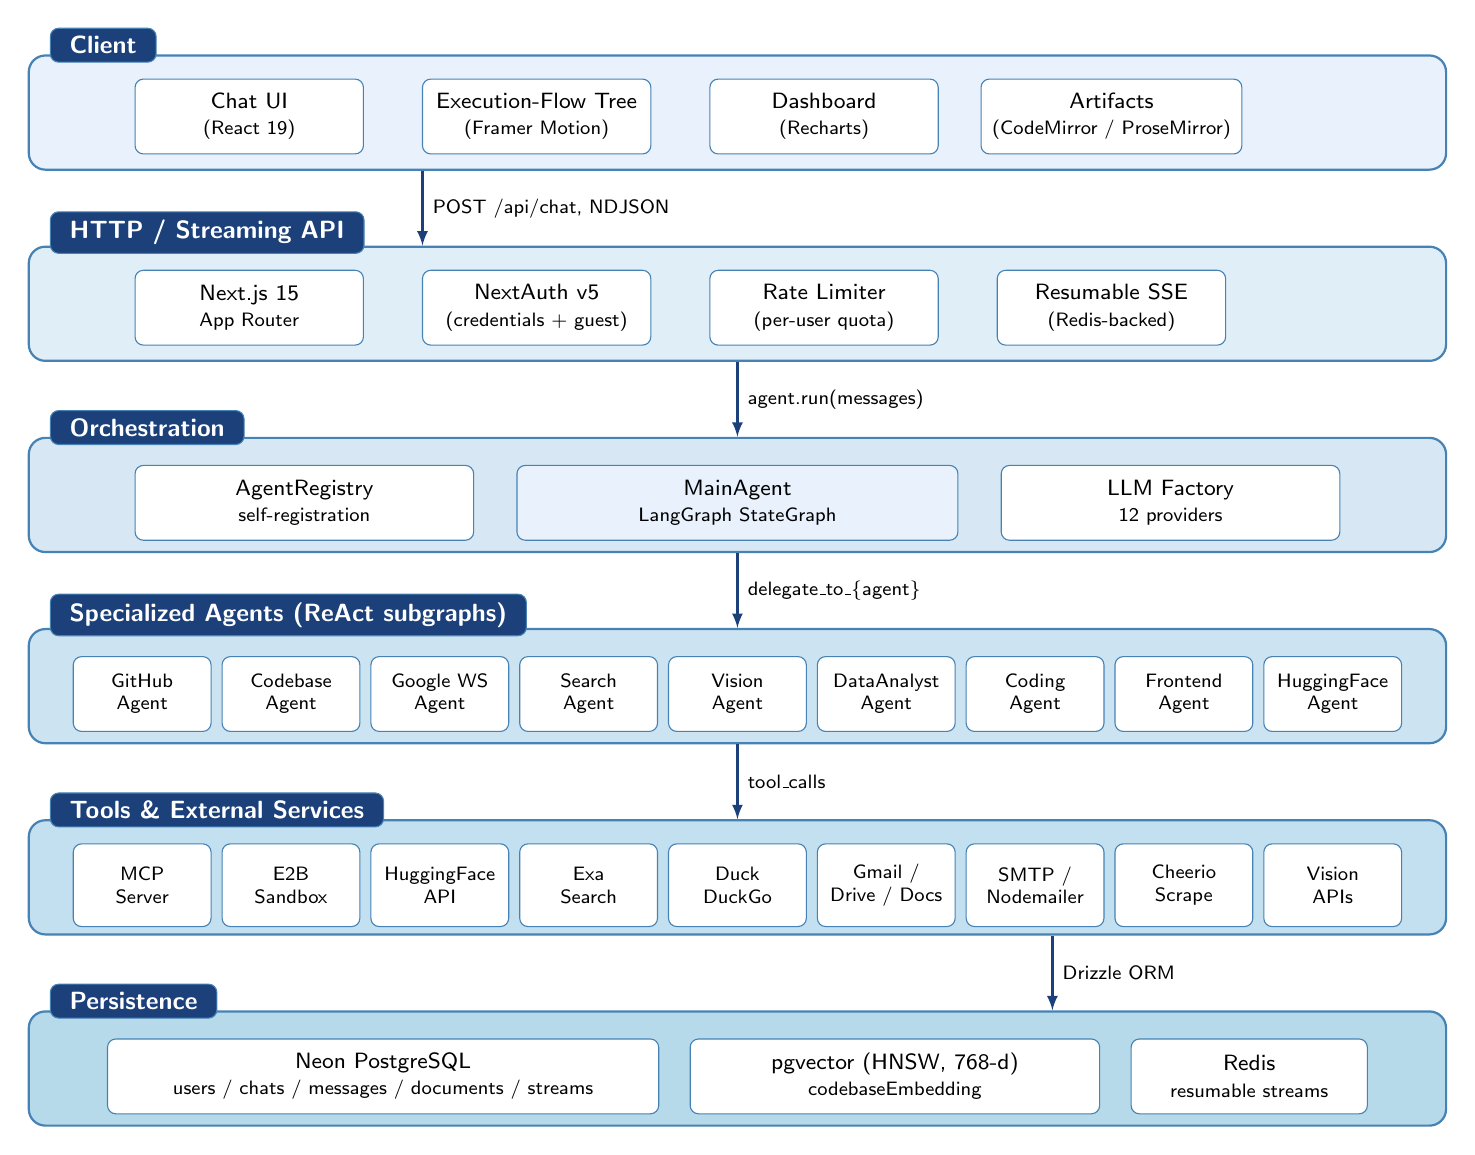
\begin{tikzpicture}[
  font=\sffamily\small,
  >=latex,
  layer/.style={
    rectangle, rounded corners=6pt, draw=BoxBorder, thick,
    inner sep=0pt, minimum height=1.45cm, minimum width=18cm, align=center
  },
  chip/.style={
    rectangle, rounded corners=3pt, draw=BoxBorder, fill=white,
    inner sep=4pt, font=\sffamily\footnotesize, align=center,
    minimum height=0.95cm, minimum width=2.9cm
  },
  lbl/.style={
    rectangle, rounded corners=3pt, draw=BoxBorder, fill=Accent,
    text=white, font=\sffamily\bfseries\small, anchor=south west,
    inner xsep=7pt, inner ysep=3pt
  },
  arrow/.style={->, thick, draw=Accent}
]

% --- CLIENT LAYER ---
\node[layer, fill=LayerClient] (client) {};
\node[lbl] at ([xshift=8pt, yshift=-3pt]client.north west) {Client};
\node[chip] at ($(client)+(-6.2,-0.05)$) {Chat UI\\\scriptsize (React 19)};
\node[chip] at ($(client)+(-2.55,-0.05)$) {Execution-Flow Tree\\\scriptsize (Framer Motion)};
\node[chip] at ($(client)+(1.1,-0.05)$) {Dashboard\\\scriptsize (Recharts)};
\node[chip] at ($(client)+(4.75,-0.05)$) {Artifacts\\\scriptsize (CodeMirror / ProseMirror)};

% --- API LAYER ---
\node[layer, fill=LayerAPI, below=0.95cm of client] (api) {};
\node[lbl] at ([xshift=8pt, yshift=-3pt]api.north west) {HTTP / Streaming API};
\node[chip] at ($(api)+(-6.2,-0.05)$) {Next.js 15\\\scriptsize App Router};
\node[chip] at ($(api)+(-2.55,-0.05)$) {NextAuth v5\\\scriptsize (credentials + guest)};
\node[chip] at ($(api)+(1.1,-0.05)$) {Rate Limiter\\\scriptsize (per-user quota)};
\node[chip] at ($(api)+(4.75,-0.05)$) {Resumable SSE\\\scriptsize (Redis-backed)};

% --- ORCHESTRATION LAYER ---
\node[layer, fill=LayerOrch, below=0.95cm of api] (orch) {};
\node[lbl] at ([xshift=8pt, yshift=-3pt]orch.north west) {Orchestration};
\node[chip, minimum width=4.3cm] at ($(orch)+(-5.5,-0.1)$) {AgentRegistry\\\scriptsize self-registration};
\node[chip, fill=LayerClient, minimum width=5.6cm] at ($(orch)+(0,-0.1)$) {MainAgent\\\scriptsize LangGraph StateGraph};
\node[chip, minimum width=4.3cm] at ($(orch)+(5.5,-0.1)$) {LLM Factory\\\scriptsize 12 providers};

% --- SPECIALIZED AGENTS ---
\node[layer, fill=LayerAgents, below=0.95cm of orch] (agents) {};
\node[lbl] at ([xshift=8pt, yshift=-3pt]agents.north west) {Specialized Agents (ReAct subgraphs)};
\foreach \i/\name in {0/GitHub, 1/Codebase, 2/{Google WS}, 3/Search, 4/Vision,
                      5/DataAnalyst, 6/Coding, 7/Frontend, 8/HuggingFace}
{
  \pgfmathsetmacro{\x}{-7.56 + \i*1.89}
  \node[chip, minimum width=1.75cm, font=\sffamily\scriptsize] at ($(agents)+(\x,-0.1)$) {\name\\\scriptsize Agent};
}

% --- TOOLS & EXTERNAL SERVICES ---
\node[layer, fill=LayerTools, below=0.95cm of agents] (tools) {};
\node[lbl] at ([xshift=8pt, yshift=-3pt]tools.north west) {Tools \& External Services};
\foreach \i/\name in {0/{MCP\\Server},1/{E2B\\Sandbox},2/{HuggingFace\\API},
                      3/{Exa\\Search},4/{Duck\\DuckGo},5/{Gmail /\\Drive / Docs},
                      6/{SMTP /\\Nodemailer},7/{Cheerio\\Scrape},8/{Vision\\APIs}}
{
  \pgfmathsetmacro{\x}{-7.56 + \i*1.89}
  \node[chip, minimum width=1.75cm, minimum height=1.05cm, font=\sffamily\scriptsize] at ($(tools)+(\x,-0.1)$) {\name};
}

% --- DATA LAYER ---
\node[layer, fill=LayerData, below=0.95cm of tools] (data) {};
\node[lbl] at ([xshift=8pt, yshift=-3pt]data.north west) {Persistence};
\node[chip, minimum width=7cm] at ($(data)+(-4.5,-0.1)$) {Neon PostgreSQL\\\scriptsize users / chats / messages / documents / streams};
\node[chip, minimum width=5.2cm] at ($(data)+(2.0,-0.1)$) {pgvector (HNSW, 768-d)\\\scriptsize codebaseEmbedding};
\node[chip, minimum width=3cm] at ($(data)+(6.5,-0.1)$) {Redis\\\scriptsize resumable streams};

% --- vertical arrows between layers ---
\draw[arrow] ($(client.south)+(-4,0)$) -- ($(api.north)+(-4,0)$)
  node[midway, right, font=\sffamily\scriptsize]{POST /api/chat, NDJSON};
\draw[arrow] ($(api.south)+(0,0)$) -- ($(orch.north)+(0,0)$)
  node[midway, right, font=\sffamily\scriptsize]{agent.run(messages)};
\draw[arrow] ($(orch.south)+(0,0)$) -- ($(agents.north)+(0,0)$)
  node[midway, right, font=\sffamily\scriptsize]{delegate\_to\_\{agent\}};
\draw[arrow] ($(agents.south)+(0,0)$) -- ($(tools.north)+(0,0)$)
  node[midway, right, font=\sffamily\scriptsize]{tool\_calls};
\draw[arrow] ($(tools.south)+(4,0)$) -- ($(data.north)+(4,0)$)
  node[midway, right, font=\sffamily\scriptsize]{Drizzle ORM};

\end{tikzpicture}%
}
\caption{Layered view of the Multi-Agent AI Framework. Each horizontal band is
a distinct concern boundary; arrows indicate the dominant request/response
path for a single user turn.}
\label{fig:arch-layered}
\end{figure}

\subsubsection*{Layered architecture walkthrough}

\begin{itemize}
  \item \textbf{Client layer.} The React~19 chat UI submits messages through a
    custom streaming handler, a collapsible execution-flow tree (powered by
    Framer Motion) visualizes live agent and tool events, a Recharts-based
    dashboard aggregates token-usage and execution metrics, and CodeMirror /
    ProseMirror power the code and document artifacts respectively.

  \item \textbf{HTTP and streaming API.} Next.js~15 App Router receives the
    request, NextAuth v5 authenticates regular or guest users, a per-user
    rate limiter enforces daily quotas, and a resumable SSE layer (backed by
    Redis) lets dropped clients re-attach to an in-flight agent run without
    losing streamed content.

  \item \textbf{Orchestration.} At module load, each specialized agent
    registers itself with the \code{AgentRegistry}. The MainAgent compiles a
    LangGraph \code{StateGraph} whose nodes are dynamically generated from
    the registry (one delegation tool and one preparation node per agent).
    The \code{createLLM(config)} factory resolves the correct LangChain chat
    client for one of twelve providers (cloud and self-hosted).

  \item \textbf{Specialized agents.} Nine domain-specific agents each run as
    an independent ReAct-style subgraph: an \code{agentNode} invokes the LLM
    with Zod-validated \code{DynamicStructuredTool}s bound, a \code{toolsNode}
    executes tool calls, and the edge condition loops until the LLM stops
    emitting tool calls.

  \item \textbf{Tools and external services.} Tools translate LLM intent into
    real-world side effects: the MCP SDK connects GitHubAgent to GitHub
    Copilot's remote MCP server, E2B runs sandboxed Python for DataAnalyst,
    Exa and DuckDuckGo provide web and semantic search, Google Workspace
    tools call Gmail / Drive / Docs / Sheets / Calendar via OAuth2, SMTP
    handles e-mail delivery, Cheerio parses scraped HTML, and the vision
    agents call OpenAI / Gemini multimodal endpoints.

  \item \textbf{Persistence.} A single Neon serverless PostgreSQL database
    stores the relational core (users, chats, messages, documents, streams)
    and the vector core (\code{codebaseEmbedding}, 768-dimensional vectors
    indexed by pgvector's HNSW operator class). Redis augments Postgres with
    ephemeral resumable-stream metadata.
\end{itemize}

\begin{figure}[H]
\centering
\resizebox{0.95\linewidth}{!}{%
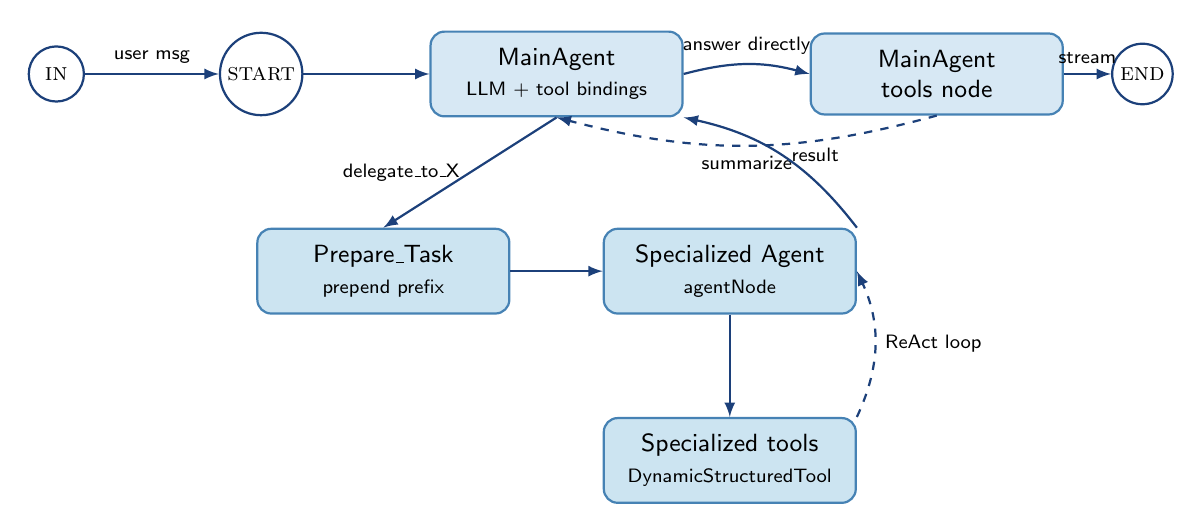
\begin{tikzpicture}[
  font=\sffamily\small,
  >=latex,
  node distance=1.2cm and 1.6cm,
  main/.style={
    rectangle, rounded corners=5pt, draw=BoxBorder, thick,
    fill=LayerOrch, align=center, inner sep=6pt, minimum height=1cm, minimum width=3.2cm
  },
  sub/.style={
    rectangle, rounded corners=5pt, draw=BoxBorder, thick,
    fill=LayerAgents, align=center, inner sep=6pt, minimum height=1cm, minimum width=3.2cm
  },
  term/.style={
    circle, draw=Accent, thick, fill=white, inner sep=2pt, minimum size=0.7cm
  },
  arrow/.style={->, thick, draw=Accent},
  loopedge/.style={->, thick, draw=Accent, dashed}
]

% Central cycle: Main agent node + tools node
\node[term] (start) {\textsc{start}};
\node[main, right=of start] (mainAgent) {MainAgent\\\scriptsize LLM + tool bindings};
\node[main, right=of mainAgent] (mainTools) {MainAgent\\tools node};

% Delegation path
\node[sub, below=1.4cm of mainAgent, xshift=-2.2cm] (prep) {Prepare\_Task\\\scriptsize prepend prefix};
\node[sub, below=1.4cm of mainAgent, xshift=2.2cm] (subAgent) {Specialized Agent\\\scriptsize agentNode};
\node[sub, below=1.3cm of subAgent] (subTools) {Specialized tools\\\scriptsize DynamicStructuredTool};

\node[term, left=of start, xshift=-0.1cm] (userin) {\textsc{in}};
\node[term, right=0.6cm of mainTools] (endnode) {\textsc{end}};

% --- edges ---
\draw[arrow] (userin) -- (start) node[midway, above, font=\sffamily\scriptsize]{user msg};
\draw[arrow] (start) -- (mainAgent);
\draw[arrow, bend left=15] (mainAgent.east) to node[above, font=\sffamily\scriptsize]{answer directly} (mainTools.west);
\draw[loopedge, bend left=15] (mainTools.south) to node[below, font=\sffamily\scriptsize]{summarize} (mainAgent.south);
\draw[arrow] (mainTools) -- (endnode) node[midway, above, font=\sffamily\scriptsize]{stream};

% Delegation branch
\draw[arrow] (mainAgent.south) -- (prep.north)
  node[midway, left, font=\sffamily\scriptsize]{delegate\_to\_X};
\draw[arrow] (prep.east) -- (subAgent.west);
\draw[arrow] (subAgent.south) -- (subTools.north);
\draw[loopedge] (subTools.north east) to[bend right=25] node[right, font=\sffamily\scriptsize]{ReAct loop} (subAgent.east);
\draw[arrow] (subAgent.north east) to[bend right=20] node[right, font=\sffamily\scriptsize]{result} (mainAgent.south east);

\end{tikzpicture}%
}
\caption{Orchestration graph for a single MainAgent invocation. Solid arrows
are deterministic transitions; dashed arrows are cycle edges driven by the
LLM's tool-call decisions.}
\label{fig:arch-langgraph}
\end{figure}

\subsubsection*{Orchestration graph walkthrough}

\begin{itemize}
  \item \textbf{Entry.} A user message enters the graph through the
    \code{START} node. The message history is passed to the MainAgent node as
    a \code{MessagesAnnotation} state.

  \item \textbf{MainAgent decision cycle.} The MainAgent LLM is bound to two
    categories of tools: direct-answer tools (artifact creation, search
    suggestions) and \code{delegate\_to\_\{agent\_id\}} delegation tools
    generated dynamically from the \code{AgentRegistry}. The conditional
    edge \code{orchestratorRoute} inspects the latest AIMessage: if it
    contains tool calls for a delegation tool, control flows into the
    corresponding subgraph; if it contains only direct tool calls, control
    flows to the local tools node; otherwise the message stream ends.

  \item \textbf{Task preparation.} Before entering a specialized subgraph,
    a small preparation node extracts the task argument from the delegation
    tool call and prepends the agent-specific task prefix (for example,
    \code{[GitHub Task]}). This keeps the specialized prompt deterministic
    and independent of how the MainAgent phrased the request.

  \item \textbf{Specialized subgraph (ReAct).} The chosen agent runs its own
    compiled graph, which is structurally identical across agents:
    \code{agentNode -> toolsNode -> agentNode}, continuing until the LLM
    stops emitting tool calls. Each tool is a Zod-validated
    \code{DynamicStructuredTool} that returns a string-serialized result;
    errors are caught and returned as text rather than thrown, so a single
    failing tool cannot collapse the parent run.

  \item \textbf{Return and summarization.} The final AIMessage of the
    specialized subgraph is lifted back into the MainAgent's state. The
    MainAgent LLM then produces a user-facing summary, which is streamed to
    the client as \code{AGENT\_STREAM} events and closed with
    \code{AGENT\_ENDED}.

  \item \textbf{Observability.} Every state transition emits structured
    events (\code{AGENT\_STARTED}, \code{TOOL\_STARTED}, \code{AGENT\_STREAM},
    \code{TOOL\_ENDED}, \code{AGENT\_ENDED}, \code{AGENT\_ERROR}) through
    LangGraph's \code{streamEvents(version: "v2")} API. The API route uses
    these events both to stream content to the browser in real time and to
    build the persisted execution tree shown in the UI.
\end{itemize}

\noindent Taken together, the two figures define the framework in the two
dimensions that matter for a production system: a \emph{horizontal} separation
of concerns across layers (clear deployment boundaries, testable units,
replaceable providers) and a \emph{vertical} state machine that remains
inspectable and deterministic even when the underlying LLM is not.

% =====================================================================
% CHAPTER 2 — Newly Used Tools and Technologies
% =====================================================================
\chapter{Newly Used Tools and Technologies}

\section{Integration of New Technologies}

The Multi-Agent AI Framework brings together a broad set of modern libraries,
protocols, and external services. Rather than relying on a single monolithic
AI SDK, the project composes purpose-built tools at each architectural layer:
agent orchestration, large-language-model (LLM) access, retrieval-augmented
generation (RAG), external service integration, web presentation, persistence,
and quality assurance. This section groups the adopted technologies by the
role they play in the system and explains how each was integrated into the
final design.

\subsection{Agent Orchestration Layer}

The orchestration layer is the backbone of the system and is built on three
newly adopted technologies.

\begin{itemize}
  \item \textbf{LangGraph} (\code{@langchain/langgraph}\ \^{}1.0.7) is used as the canonical state-graph engine. The MainAgent and all nine specialized agents are compiled into a \code{StateGraph} with \code{MessagesAnnotation} as the shared state type. LangGraph replaces the classical request--response loop with a stateful, cyclic execution model, in which an \code{agentNode} $\rightarrow$ \code{tools} $\rightarrow$ \code{agentNode} cycle drives tool-calling until the LLM decides to terminate the conversation. This enables deterministic tool execution, explicit routing, and the real-time execution-flow visualization displayed to the user.
  \item \textbf{LangChain Core} (\code{@langchain/core}\ \^{}1.1.8) provides the \code{DynamicStructuredTool}, \code{BaseMessage}, and \code{Runnable} contracts that every agent tool adheres to. All 88+ tools in the framework share a common Zod-validated signature thanks to this abstraction, which makes tools portable between agents and predictable at the LLM-invocation boundary.
  \item \textbf{Model Context Protocol (MCP) SDK} (\code{@modelcontextprotocol/sdk}\ \^{}1.25.1) is adopted by the GitHubAgent, which connects to GitHub Copilot's remote MCP server through \code{StreamableHTTPClientTransport}. MCP is a very recent (2024--2025) standard for exposing tool servers to LLM clients, and its use in this project represents an early and successful adoption of an emerging industry protocol.
\end{itemize}

\subsection{Large Language Model Providers}

A \textbf{provider-agnostic LLM factory} (\code{lib/agents/llmFactory.ts})
decouples agent logic from any specific vendor. Twelve providers are
supported, allowing users to switch between cloud, self-hosted, and fully
custom endpoints at runtime.

\begin{longtable}{@{}L{2.3cm} L{4.8cm} L{6.6cm}@{}}
\toprule
\textbf{Category} & \textbf{Provider} & \textbf{Package / Endpoint}\\
\midrule\endhead
Cloud        & Google Gemini         & \code{@langchain/google-genai}\\
Cloud        & OpenAI                & \code{@langchain/openai}\\
Cloud        & Groq                  & \code{@langchain/groq}\\
Cloud        & Anthropic (Claude)    & \code{@langchain/anthropic}\\
Cloud        & Mistral               & \code{@langchain/mistralai}\\
Cloud        & Ollama Cloud          & \code{@langchain/ollama} with authorization headers\\
Self-hosted  & Ollama (local)        & \code{@langchain/ollama}\\
Self-hosted  & LM Studio             & OpenAI-compatible endpoint, \code{localhost:1234}\\
Self-hosted  & LocalAI               & OpenAI-compatible endpoint, \code{localhost:8080}\\
Self-hosted  & llama.cpp             & OpenAI-compatible endpoint, \code{localhost:8000}\\
Self-hosted  & text-generation-webui & OpenAI-compatible endpoint, \code{localhost:5000}\\
Custom       & Any OpenAI-compatible & User-supplied \code{baseURL}\\
\bottomrule
\end{longtable}

This multi-provider support is itself a non-trivial piece of infrastructure:
each provider exposes distinct authentication, streaming semantics, and
tool-calling dialects, all reconciled behind a single \code{createLLM(config)}
call. The unit-test suite for this factory alone validates Google-key
enforcement, OpenAI client creation with base-URL support, fallback behavior
for OpenAI-compatible servers, Ollama Cloud authorization, and rejection of
unknown providers.

\subsection{Retrieval-Augmented Generation Stack}

\begin{itemize}
  \item \textbf{pgvector} (via Drizzle ORM\ \^{}0.34.0 over Neon serverless PostgreSQL) stores 768-dimensional embeddings in the \code{codebaseEmbedding} table. An \textbf{HNSW (Hierarchical Navigable Small World)} index with cosine distance provides approximate nearest-neighbor search at $O(\log n)$ complexity, enabling sub-second semantic lookup even over large codebases.
  \item \textbf{Google \code{text-embedding-004}} is used to embed both indexed code chunks and natural-language user queries. Using a single embedding model on both sides keeps the vector space consistent and avoids domain drift between indexer and retriever.
  \item A \textbf{custom TypeScript/Python AST chunker} splits source files by function, class, method, and import declarations rather than by na\"ive line or token count. This semantically aware chunking is essential for retrieval precision on source code, which has very different structural properties from natural-language documents.
\end{itemize}

\subsection{External Service Integrations}

\begin{itemize}
  \item \textbf{Google Workspace APIs (OAuth2)} --- Gmail, Google Drive, Google Docs, Google Sheets, Google Slides, and Google Calendar are exposed through 27 tools across six services in the GoogleWorkspaceAgent.
  \item \textbf{E2B Code Interpreter} (\code{@e2b/code-interpreter}\ \^{}2.3.3) provides a secure, sandboxed Python environment used by the DataAnalystAgent to execute pandas/numpy/matplotlib code without exposing the host system to untrusted scripts.
  \item \textbf{HuggingFace Inference API} (\code{@huggingface/inference}\ \^{}4.13.10) powers the HuggingFaceAgent's nine tools (model inference, model search, dataset search, paper search, spaces exploration, documentation search, repository details).
  \item \textbf{Exa API} (\code{exa-js}\ \^{}2.0.12) performs semantic web and academic-paper search for the SearchAgent.
  \item \textbf{DuckDuckGo} (\code{duck-duck-scrape}\ \^{}2.2.7) provides general web, news, and image search without requiring an API key.
  \item \textbf{Cheerio} (\code{cheerio}\ \^{}1.1.2) is used for server-side HTML parsing and DOM traversal when the SearchAgent extracts content from fetched URLs.
  \item \textbf{Nodemailer} (\code{nodemailer}\ 6.9.15) provides SMTP delivery for the legacy EmailAgent, with an \code{EMAIL\_DRY\_RUN} mode that allows safe end-to-end testing without sending real mail.
  \item \textbf{ngrok + Google Colab} forms a novel deployment pattern that exposes a Colab-hosted Ollama instance as a public HTTPS endpoint, allowing free-tier GPU inference to serve the application.
\end{itemize}

\subsection{Web and Frontend Platform}

\begin{itemize}
  \item \textbf{Next.js 15} (\code{next}\ 15.6.0-canary.58, Turbopack mode) provides the App Router, server actions, middleware-based authentication, and streaming responses implemented over \code{ReadableStream}.
  \item \textbf{React 19} (release candidate) is used for concurrent rendering of the streaming chat UI and the collapsible \code{ExecutionFlowComponent}.
  \item \textbf{Tailwind CSS v4, Radix UI primitives, and shadcn-style components} form the design-system foundation.
  \item \textbf{Framer Motion} (\code{framer-motion}\ \^{}11.3.19) animates the collapsible execution-flow tree and other UI transitions.
  \item \textbf{CodeMirror 6} provides syntax-highlighted code artifacts, with JavaScript and Python language packs integrated.
  \item \textbf{ProseMirror} powers rich-text editing for document artifacts.
  \item \textbf{Recharts} (\code{recharts}\ \^{}3.6.0) renders the data visualizations on the user dashboard.
  \item \textbf{Shiki} and \textbf{streamdown} handle static code rendering and streaming-markdown output respectively.
\end{itemize}

\subsection{Persistence, Authentication, and Streaming}

\begin{itemize}
  \item \textbf{Drizzle ORM + Neon serverless PostgreSQL} (\code{@neondatabase/serverless}\ \^{}1.0.2) provides type-safe database access, schema migrations, and edge-compatible connection pooling.
  \item \textbf{NextAuth v5} (\code{next-auth}\ 5.0.0-beta.25) implements two-credential-provider authentication (regular user and guest) with JWT-based sessions.
  \item \textbf{bcrypt-ts} hashes user passwords.
  \item \textbf{Redis} (\code{redis}\ \^{}5.0.0) combined with \textbf{\code{resumable-stream}}\ \^{}2.0.0 provides optional resumable server-sent event streams, so that dropped client connections can reattach to an in-flight agent run without losing context.
  \item \textbf{Zod} (\code{zod}\ \^{}3.25.76) performs runtime validation at every boundary: tool input schemas, API request bodies, and environment-configuration objects.
\end{itemize}

\subsection{Testing, Observability, and Quality Tooling}

\begin{itemize}
  \item \textbf{Playwright}\ \^{}1.50.1 drives end-to-end browser automation, covering 48 E2E scenarios across authentication, chat, artifacts, reasoning, session persistence, and user isolation.
  \item \textbf{Vitest}\ \^{}4.0.18 is the unit- and integration-test runner, hosting 296 unit tests, 108 route/contract tests, and the integration tests for orchestrator delegation.
  \item \code{@vitest/coverage-v8} produces code-coverage reports.
  \item \textbf{Ultracite} and \textbf{Biome} (\code{@biomejs/biome}\ 2.2.2) form the linting and formatting pipeline.
  \item \textbf{TypeScript 5.6} is used in strict mode, with generics and discriminated unions encoding message types.
  \item \textbf{OpenTelemetry} (\code{@opentelemetry/api}, \code{@vercel/otel}) provides structured tracing hooks available for production observability.
  \item \textbf{TokenLens}\ 1.3.0 performs per-provider token counting and feeds the dashboard's usage metrics.
\end{itemize}

\subsection{Why These Choices Matter}

The combination above is deliberately \textbf{poly-provider, poly-protocol,
and poly-model}. LangGraph gives deterministic state control where raw
streaming would be ad hoc; MCP offers a forward-compatible way to add tool
servers without bespoke clients; pgvector keeps the RAG stack inside the main
transactional database, eliminating the operational overhead of a separate
vector store; and the twelve-provider factory insulates the project from
vendor instability, pricing changes, and region-specific compliance
constraints.

Taken together, these technologies make the framework a concrete exercise in
integrating \textbf{newly emerging AI standards} (MCP, LangGraph,
pgvector-based RAG, streaming multi-agent orchestration) with \textbf{mature
web-platform primitives} (Next.js, PostgreSQL, NextAuth, OAuth2). The result
is a system that can evolve with the rapidly moving AI ecosystem without
discarding the well-understood guarantees of conventional web engineering.

% =====================================================================
% CHAPTER 3 — Impacts of the Engineering Solutions
% =====================================================================
\chapter{Impacts of the Engineering Solutions}

The developed multi-agent artificial intelligence framework goes beyond being
merely a technical software project and produces significant effects in
economic, environmental, and societal dimensions. This chapter examines these
impacts in detail.

\section{Economic Impacts}

The economic impact of multi-agent AI systems can be analyzed at both micro
and macro levels. At the micro level, such systems enable businesses to
automate repetitive information-processing tasks, thereby reducing
human-resource costs and allowing employees to focus on more creative,
high-value-added work. For example, the project's specialized modules such as
the email agent and coding agent are concrete manifestations of this type of
task automation.

At the macro level, the rapid proliferation of platforms based on large
language models is contributing to the dramatic growth of the AI services
market. Indeed, the global AI market is projected to exceed 1.8 trillion
dollars by 2030. However, the economic benefits of this growth are not
distributed equally. The dominance of a few major technology companies such
as OpenAI, Anthropic, and Google in the market can increase access costs for
small and medium-sized enterprises. This project aims to mitigate that
monopolization risk, to some extent, by integrating multiple LLM providers
(OpenAI, Anthropic, Google Gemini, Groq, Ollama, etc.) within a single
framework; users can switch between different providers according to the
cost-performance balance that suits them.

On the other hand, support for local and open-source models through Ollama
integration reduces dependence on cloud-based APIs and offers an economically
sustainable alternative, especially for developers and small teams facing
continuous API-usage costs. This approach has a democratizing economic impact
by making artificial intelligence accessible to a broader audience.

\section{Environmental Impacts}

The environmental cost of training and operating large language models is
becoming an increasingly prominent area of concern. The energy consumed
during the training of large-scale language models such as GPT-4 is
estimated to be in the hundreds of megawatt-hours. Against this background,
the environmental impact of the developed framework must be evaluated from
two perspectives.

\paragraph{Positive environmental impacts.}
The project uses pre-trained models in the inference phase rather than
retraining them from scratch. This approach significantly reduces the carbon
footprint compared with training a model from the ground up. In addition,
thanks to the Ollama integration, models can run on the user's local
hardware, eliminating the need to route every user request to large data
centers; this reduces both energy consumption and the indirect carbon
emissions arising from network communication. Furthermore, Next.js's
server-side rendering (SSR) and partial prerendering (PPR) features minimize
unnecessary client-side computations and contribute to energy efficiency at
the edge.

\paragraph{Negative environmental impacts.}
On the other hand, the system's simultaneous use of multiple agents and LLM
providers consumes more computational resources than a single-model call.
Parallel processing of tasks in the multi-agent architecture increases CPU
and GPU usage, contributing to the power consumption of data centers. In the
long term, this effect may become more pronounced as these systems scale.

In conclusion, for environmentally friendly AI usage, energy efficiency
should also be considered a criterion in model selection, and local or
smaller, more efficient models should be preferred whenever possible.

\section{Societal and Global Impacts}

The societal and global impacts of multi-agent artificial intelligence
systems should be evaluated from a much broader perspective than their
technical characteristics.

\paragraph{Accessibility and the digital divide.}
This project facilitates access to artificial intelligence independent of
technological infrastructure by unifying different LLM providers under a
single interface. In particular, support for open-source models (via Ollama)
offers a significant opportunity for developers and educational institutions
in developing countries that cannot afford high-cost commercial APIs. From
this standpoint, the project has the potential to narrow the digital divide
in the field of artificial intelligence.

\paragraph{Employment and workforce transformation.}
Multi-agent automation systems have the capacity to automate certain
knowledge-worker tasks. Specialized modules such as the coding agent, email
agent, and vision agent have the potential to transform work processes in
areas such as software development, customer communication, and image
analysis. While this may lead to the automation of some routine tasks, it
also creates demand for new skills (managing, supervising, and improving AI
systems).

\paragraph{Education and access to knowledge.}
The system has the potential to accelerate access to information through its
codebase-indexing and document-processing capabilities. Educational
institutions and researchers can use such systems to increase academic
productivity in complex knowledge-management tasks.

\paragraph{Global competition and technological sovereignty.}
The capacity to develop multi-agent AI infrastructure is becoming an
increasingly important element of competition between countries and
companies. The project's open-source philosophy and multi-provider support
promote technological independence without dependence on any specific
geography or provider. This approach addresses the ``vendor lock-in'' problem,
which has gained importance in discussions of technological sovereignty.

% =====================================================================
% CHAPTER 4 — Current Issues Related to the Project Field
% =====================================================================
\chapter{Current Issues Related to the Project Field}

\section{Current Discussions in the Field}

Large language models and multi-agent artificial-intelligence systems have
been at the center of both academic and industrial discussions between 2023
and 2025. These discussions formed a decisive context during the development
of the project.

\paragraph{Hallucination and reliability.}
One of the most debated limitations of large language models is their
tendency to produce ``hallucinations''---information presented as factual but
lacking accuracy. This project aims to reduce the model's dependence on its
own contextual knowledge by using the RAG (Retrieval-Augmented Generation)
architecture and the codebase-indexing module. However, completely
eliminating the hallucination problem remains an unsolved research issue.

\paragraph{AI safety and alignment.}
Efforts to ensure that AI systems behave in accordance with human values---
known as ``alignment'' research---constitute one of today's most critical AI
agendas. Anthropic's Constitutional AI approach and OpenAI's safety layers
are practical reflections of this discussion. In this project's system
architecture, respect has been shown for the safety layers of Anthropic
Claude and other models; design decisions have been made to limit the scope
and authority of agent actions.

\paragraph{Data privacy and GDPR compliance.}
The storage and processing of user conversation history in the database lie
at the heart of data-privacy discussions. In Europe, GDPR, and in the United
States, evolving state-level data-protection laws are regulating more
strictly how AI systems can collect and store user data. Although this
project uses NextAuth.js for authentication and secure session management,
establishing a clear policy on how user data is processed and ensuring
compliance with GDPR requirements remains a critical priority for future
development.

\paragraph{Controllability in multi-agent systems.}
In systems where multiple AI agents operate simultaneously, answering the
question ``which agent made which decision and why?'' is becoming increasingly
difficult. This ``explainability'' issue is on the agenda of both academic
research and regulatory bodies. The European Union AI Act requires certain
high-risk AI applications to be explainable and auditable. The
LangGraph-based agent orchestration in this project provides a practical
response to this discussion by offering logging and monitoring infrastructure
for each agent's actions.

\paragraph{Tension between open-source and closed-source models.}
The rise of Meta's LLaMA series, Mistral, and other open-source models has
sparked a deep debate in the AI community. While open-source advocates
highlight the democratizing effect and research transparency of these
models, closed-source proponents emphasize security risks and potential for
misuse. This project acts as a neutral bridge in this discussion through its
multi-provider architecture that draws the best from both worlds.

\paragraph{Artificial intelligence and copyright.}
The copyright status of training data and the intellectual-property status of
content generated by AI are subject to legal proceedings worldwide. The
\emph{New York Times} lawsuit against OpenAI and Getty Images' legal actions
against image-generation models are among the most prominent examples of
this discussion. The usage conditions and liability status of content
produced within this project are critical issues that must be legally
evaluated before real-world distribution.

% =====================================================================
% CHAPTER 5 — Background Research and Use of Sources
% =====================================================================
\chapter{Background Research and Use of Sources}

\section{Similar Designs and Component Information}

During the design phase the team investigated several prior-art directions.
Each of them influenced a concrete architectural decision in the final
system, and together they provide the intellectual scaffolding on which the
implementation rests.

\subsection{Multi-Agent Orchestration Frameworks}

\begin{itemize}
  \item \textbf{LangGraph} (LangChain Inc., 2024) was adopted directly. Its \code{StateGraph} with \code{MessagesAnnotation} was chosen because it offers explicit, inspectable control flow, unlike the implicit ReAct loops found in earlier LangChain \code{AgentExecutor} designs. This explicitness is what makes the project's execution-flow visualization feasible.
  \item \textbf{Microsoft AutoGen} (Wu et al., 2023) was studied for its conversational multi-agent model and group-chat orchestrator. AutoGen inspired the idea of a central orchestrator (the MainAgent) dispatching work to specialist agents. However, the framework diverges by making delegation an \emph{LLM tool call} rather than a free-form conversation, yielding stricter task boundaries and easier auditability.
  \item \textbf{CrewAI} was reviewed for its role-based agent design. While CrewAI organizes agents by persona (``researcher'', ``writer'', etc.), this project organizes them by \emph{domain capability and tool surface}. That alignment fits better with the plugin-style \code{AgentRegistry} used here, where each specialized agent is defined by the set of tools it exposes.
  \item \textbf{AutoGPT} and \textbf{BabyAGI} (2023) were studied as early autonomous-agent prototypes. Their unbounded self-planning loops motivated the design decision to keep the MainAgent's delegation scope explicit, tool-bounded, and observable, avoiding the reliability and cost issues that plagued those systems.
\end{itemize}

\subsection{Foundational Academic Work on LLM Agents}

\begin{itemize}
  \item \textbf{Yao et al., ``ReAct: Synergizing Reasoning and Acting in Language Models,''} NeurIPS 2022 (arXiv:2210.03629) --- the foundational paper for interleaved reasoning and tool use. The \code{agentNode} $\rightarrow$ \code{tools} $\rightarrow$ \code{agentNode} cycle inside every LangGraph subgraph in this project is a direct instantiation of the ReAct pattern.
  \item \textbf{Lewis et al., ``Retrieval-Augmented Generation for Knowledge-Intensive NLP Tasks,''} NeurIPS 2020 (arXiv:2005.11401) --- the canonical RAG paper. The CodebaseAgent's indexer, embedder, and retriever form a classical RAG pipeline specialized for source code rather than natural-language documents.
  \item \textbf{Malkov and Yashunin, ``Efficient and Robust Approximate Nearest Neighbor Search using Hierarchical Navigable Small World Graphs,''} IEEE TPAMI 2018 (arXiv:1603.09320) --- the algorithm backing the pgvector \code{hnsw} index used for cosine-similarity search over 768-dimensional embeddings.
  \item \textbf{Vaswani et al., ``Attention Is All You Need,''} NeurIPS 2017 (arXiv:1706.03762) --- the underlying Transformer architecture on which every integrated LLM ultimately depends.
  \item \textbf{Schick et al., ``Toolformer: Language Models Can Teach Themselves to Use Tools,''} NeurIPS 2023 (arXiv:2302.04761) --- background reading on tool-augmented LLMs, relevant to the design of the \code{DynamicStructuredTool} abstraction.
  \item \textbf{Brown et al., ``Language Models are Few-Shot Learners,''} NeurIPS 2020 (arXiv:2005.14165) --- the GPT-3 paper that motivates the few-shot prompt structure used by the MainAgent's delegation prompts.
\end{itemize}

\subsection{Protocols, Standards, and Vendor Documentation}

\begin{itemize}
  \item The \textbf{Model Context Protocol (MCP) specification} (Anthropic, 2024--2025) was followed exactly as published: \code{StreamableHTTPClientTransport} connects the GitHubAgent to GitHub Copilot's hosted MCP server, and tool calls are marshaled through the SDK rather than re-implemented.
  \item \textbf{OpenAI Function Calling and Tool Use documentation} informed the schema format used by \code{DynamicStructuredTool} (JSON Schema derived automatically from Zod objects).
  \item \textbf{Anthropic Claude Tool Use and Constitutional AI documentation} was consulted when configuring safety-aware agents and when studying the alignment practices discussed in Chapter~4.
  \item \textbf{Google Generative AI / Gemini API documentation} was the primary reference for the default MainAgent provider and for the \code{text-embedding-004} model used by the RAG pipeline.
  \item \textbf{LangChain.js and LangGraph.js official documentation} (\url{https://js.langchain.com}, \url{https://langchain-ai.github.io/langgraphjs}) was the single most-consulted source during day-to-day implementation.
\end{itemize}

\subsection{Web Platform and Infrastructure References}

\begin{itemize}
  \item \textbf{Next.js 15 official documentation} (\url{https://nextjs.org/docs}) --- App Router, streaming responses, server actions, and middleware patterns.
  \item \textbf{Drizzle ORM documentation} (\url{https://orm.drizzle.team}) --- schema definitions, migrations, and pgvector integration.
  \item \textbf{Neon serverless PostgreSQL documentation} --- connection pooling and edge-compatible drivers.
  \item \textbf{NextAuth.js v5 (Auth.js) documentation} --- credential providers, JWT-based sessions, middleware-based route protection.
  \item \textbf{E2B Code Interpreter documentation} --- sandboxed Python execution semantics.
  \item \textbf{HuggingFace Inference API reference} --- model invocation semantics and rate-limit behavior.
  \item \textbf{pgvector README and SQL reference} --- HNSW index parameters and cosine-distance operators.
  \item \textbf{Vercel AI SDK documentation} --- consulted for comparison; the project intentionally implements its own JSON-event streaming protocol instead of using Vercel's \code{useChat} hook, in order to preserve fine-grained control over execution-flow event ordering.
\end{itemize}

\subsection{How Prior Art Was Adapted}

The novelty of the project lies less in any single component than in how
components are \textbf{composed}. The following adaptations are explicit
contributions of this work:

\begin{enumerate}
  \item A self-registering \code{AgentRegistry} --- inspired by plugin systems such as VS Code extensions and Express middleware registries --- replaces the hard-coded agent list found in tutorial-grade LangGraph examples.
  \item The \textbf{delegation-as-tool-call} pattern takes the ``handoff'' idea from multi-agent chat frameworks and implements it as a schema-validated tool invocation, which keeps the orchestration LLM-driven while remaining type-safe and auditable.
  \item A twelve-provider LLM factory generalizes the two- or three-provider abstractions found in most LangChain tutorials, with explicit handling of both cloud APIs and OpenAI-compatible self-hosted servers (LM Studio, llama.cpp, LocalAI, text-generation-webui, custom vLLM endpoints).
  \item \textbf{RAG over source code}, rather than over documents, required custom TypeScript and Python chunking logic, because off-the-shelf document loaders chunk on paragraph or sentence boundaries that are unsuitable for code structure.
  \item The \textbf{Colab + Ollama + ngrok} deployment recipe is a pragmatic adaptation inspired by the self-hosted LLM community; no single formal publication describes it, so the project contributes its own working documentation.
\end{enumerate}

\section{Fundamental Engineering Principles and Lifelong Learning}

\subsection{Engineering Principles Applied}

The codebase consciously reflects well-established software-engineering
principles, each of which has observable consequences in the final
architecture.

\paragraph{SOLID principles.}
\begin{itemize}
  \item \emph{Single responsibility} --- each agent owns exactly one domain (GitHub, Codebase, Email, Vision, Data Analysis, \ldots); the registry, the LLM factory, and the configuration resolver are each single-purpose modules.
  \item \emph{Open/closed} --- new agents are added without modifying the MainAgent; they self-register with \code{agentRegistry.register(\ldots)}. The orchestration layer is open for extension, closed for modification.
  \item \emph{Liskov substitution} --- every agent is interchangeable through the \code{BaseAgent<T>} abstraction; the MainAgent treats all specialized agents uniformly.
  \item \emph{Interface segregation} --- tools are narrow, purpose-specific \code{DynamicStructuredTool} instances rather than one god-class per agent.
  \item \emph{Dependency inversion} --- agents depend on the abstract \code{createLLM} factory rather than on any concrete provider SDK.
\end{itemize}

\paragraph{Design patterns.}
\begin{itemize}
  \item \emph{Factory pattern} --- \code{createLLM(config)} selects the appropriate LangChain chat client at runtime.
  \item \emph{Registry pattern} --- \code{AgentRegistry} is the single source of truth for available agents.
  \item \emph{Strategy pattern} --- each provider branch inside \code{createLLM} is an interchangeable strategy.
  \item \emph{Observer / event-stream pattern} --- the JSON event stream (\code{AGENT\_STARTED}, \code{TOOL\_STARTED}, \code{AGENT\_STREAM}, \code{TOOL\_ENDED}, \code{AGENT\_ENDED}, \code{AGENT\_ERROR}) implements a lightweight publish/subscribe channel that decouples the agent runtime from the UI.
  \item \emph{Template method} --- \code{BaseAgent} defines the orchestration skeleton and delegates domain logic to its subclasses' tool sets.
  \item \emph{Composition over inheritance} --- agents compose tools rather than subclassing specialized agent base classes.
\end{itemize}

\paragraph{Architectural principles.}
\begin{itemize}
  \item \emph{Separation of concerns} --- configuration, prompt, tools, and agent class live in separate files inside each \code{lib/agents/<name>/} directory.
  \item \emph{Plugin architecture} --- the self-registration pattern is a textbook plugin system.
  \item \emph{Twelve-factor-app influences} --- all credentials are stored in environment variables; the application is stateless at the HTTP layer; logs are structured event streams.
  \item \emph{Defense in depth} --- Zod validates at tool boundaries; NextAuth guards the HTTP boundary; rate-limiting guards per-user usage; \code{EMAIL\_DRY\_RUN} guards destructive external side effects.
\end{itemize}

\paragraph{Data and algorithmic principles.}
\begin{itemize}
  \item \emph{Normalization and relational integrity} in the PostgreSQL schema (\code{user}, \code{chat}, \code{message}, \code{vote}, \code{document}, \code{suggestion}, \code{stream}).
  \item \emph{Approximate nearest-neighbor search (HNSW)} providing sub-linear $O(\log n)$ retrieval over vector data.
  \item \emph{Idempotency and deterministic hashing} in the configuration resolver; a \code{configVersion} key avoids rebuilding the LLM and tool set when nothing has changed.
  \item \emph{Graceful degradation} --- every tool returns an error string rather than throwing, so a single tool failure cannot collapse an entire agent run.
\end{itemize}

\paragraph{Security and privacy principles.}
\begin{itemize}
  \item \emph{Principle of least privilege} --- the GitHub personal access token, SMTP credentials, and OAuth tokens are scoped and isolated per agent.
  \item \emph{Encryption at rest} for per-user agent configurations (verified by the \code{encryption} and \code{configResolver} unit tests).
  \item \emph{Input validation at every boundary} via Zod.
  \item \emph{User isolation} --- chats, votes, preferences, analytics, and streams are all explicitly tested for cross-user isolation in the route/contract suites.
\end{itemize}

\subsection{Lifelong Learning and Self-Directed Study}

Completing this project required the team to engage in substantial
self-directed learning, because the technology frontier moved faster than
any textbook could keep up with. Specific examples include:

\begin{itemize}
  \item Studying frameworks released within the last twelve months, including LangGraph 1.x (a ground-up rewrite of the legacy \code{AgentExecutor}), LangChain 1.x, Next.js 15's App Router and Turbopack, and React 19's concurrent features.
  \item Tracking an emerging standard --- MCP --- from specification to production integration within the same development cycle, including reading the protocol's RFC-style documents and the reference SDK.
  \item Cross-domain learning --- database indexing theory (HNSW), vector embeddings, OAuth2, SMTP, streaming HTTP semantics, and browser-level testing (Playwright). Few of these topics are typically taught together in a single undergraduate course.
  \item Reading primary academic literature (ReAct, RAG, HNSW, Transformer) to understand \emph{why} the tools behave the way they do, not merely \emph{how} to call them.
  \item Benchmarking and comparative study of cloud versus self-hosted LLMs, which led directly to the deliberate decision to support twelve providers and to document the Colab + ngrok deployment recipe for users without GPU access.
  \item Learning testing as a discipline --- building a 486-test matrix across five complementary layers (unit, integration, end-to-end, route/contract, and performance) required adopting Vitest, Playwright, and contract-testing methodology, all of which extended the team's prior testing vocabulary.
  \item Community engagement --- project decisions were informed by LangChain GitHub issues, Next.js discussions, pgvector mailing lists, and Anthropic/OpenAI developer forums. The ability to locate authoritative answers quickly, cross-reference them, and integrate them into a working system is itself a lifelong-learning competency.
\end{itemize}

This combination of \textbf{timeless engineering principles} (SOLID, design
patterns, separation of concerns) and \textbf{continuous adaptation to a
rapidly moving AI ecosystem} reflects the accredited engineering-education
expectation that graduates must ``recognize the need for and engage in
lifelong learning.'' The project is therefore not only a technical artifact,
but also a demonstration of the learning practices required to build and
maintain such an artifact in a fast-evolving field.

% =====================================================================
% CHAPTER 6 — Test Results and Evaluation
% =====================================================================
\chapter{Test Results and Evaluation}

The final validation stage confirmed that the project achieved a fully
successful automated test baseline. In the last verified run, all official
automated tests passed, demonstrating that the system behaved correctly
across its major technical layers. The validated matrix contains 486 unique
automated tests distributed across 54 executed suites. These tests are
organized into five complementary categories: unit testing, integration
testing, end-to-end testing, route and contract testing, and performance
testing.

From an engineering standpoint, this layered structure significantly
increases confidence in the reliability of the application. Unit tests
verify the correctness of the project's smallest functional elements,
including agent definitions, factories, registries, encryption logic,
configuration handling, utilities, and document-related operations. These
tests ensure that the internal building blocks of the system behave as
expected in isolation. Integration tests extend this validation by
confirming that the orchestration mechanism of the system works properly,
particularly that the main agent can delegate tasks to specialized sub-agents
and receive coherent results in return. This is especially relevant in a
multi-agent architecture, where correct coordination is just as important as
the correctness of the individual components.

End-to-end tests provide a different but equally important perspective.
Rather than focusing on isolated functions or internal service contracts,
they validate the system from the viewpoint of a real user interacting
through the browser. These tests cover practical workflows such as
authentication, guest access, registration, login, conversation persistence,
chat creation, message interaction, artifact generation, reasoning
visibility, and user isolation. As a result, they demonstrate that the
application is not only technically correct at the code level, but also
usable and consistent as a complete interactive product.

The route- and contract-test layer strengthens the evaluation further by
focusing on API correctness and system boundaries. These tests verify
request validation, expected response structures, authorization behavior,
per-user data isolation, streaming semantics, and endpoint-specific business
rules. In a project where persistent conversations, user-specific settings,
analytics, metrics, voting, and multimodal interactions are handled through
API endpoints, this layer is essential. It ensures that the application does
not only produce correct outputs under ideal conditions, but also enforces
proper access control and data separation under realistic usage scenarios.

The inclusion of a dedicated performance layer makes the evaluation more
comprehensive than a conventional functional-test report. Performance tests
assess route latency, encrypted configuration throughput, history-query
behavior under varying loads, and streaming responsiveness metrics such as
time-to-first-chunk and total stream-completion time. These checks are
valuable because a conversational multi-agent application must not only be
correct, but also responsive enough to support a satisfactory user
experience.

The fact that all validated tests passed means that the system satisfied
correctness requirements at the code level, orchestration requirements at
the architectural level, usability expectations at the interface level,
contract requirements at the API level, and responsiveness requirements at
the operational level.

\section{Test Cases}

Table~\ref{tbl:test-cases} consolidates the executed test suites and the
concrete scenarios validated inside each suite. Each row corresponds to an
executed suite in the final matrix, and the scenario descriptions summarize
the complete set of validated test cases covered by that suite.

{\footnotesize\setlength{\tabcolsep}{3.5pt}
\begin{longtable}{@{}L{1.6cm} L{3.2cm} L{5.45cm} L{3.15cm} L{1.1cm}@{}}
\caption{Executed test suites and scenarios.}\label{tbl:test-cases}\\
\toprule
\textbf{Layer} & \textbf{Executed Test Suite} & \textbf{Covered Test Cases and Scenarios} & \textbf{Evaluation Focus} & \textbf{Status}\\
\midrule\endfirsthead
\multicolumn{5}{c}{\textit{(continued)}}\\
\toprule
\textbf{Layer} & \textbf{Executed Test Suite} & \textbf{Covered Test Cases and Scenarios} & \textbf{Evaluation Focus} & \textbf{Status}\\
\midrule\endhead
Unit & AgentRegistry & Registration and retrieval by identifier; retrieval by tool name; full registry listing; registry-size tracking; duplicate-identifier overwrite behavior & Central agent registration and lookup mechanics & Passed\\
Unit & Artifact-server contract & Alignment between artifact kinds and document handlers; persistence of newly created content for sessions with a user identifier; safe no-persist behavior without a session user; persistence of updated content with existing document metadata & Artifact lifecycle consistency and persistence rules & Passed\\
Unit & BaseAgent & Exposure of agent identifier and name from configuration metadata; compiled-graph construction; response generation as a readable stream & Common execution contract shared by all agents & Passed\\
Unit & CodebaseAgent Tools & Non-empty tool creation; tool-metadata integrity; \code{search\_codebase} tool definition; successful invocation; result-path correctness; file-path prefix filtering; result limiting; no-result behavior; graceful fallback on vector-search failure & Codebase retrieval tooling and search robustness & Passed\\
Unit & Codebase chunking core & Extraction of imports, functions, arrow functions, and interfaces from TypeScript; oversized-class splitting into overview and method chunks; fallback line-based chunking for non-TypeScript files & Indexing and chunk-preparation logic behind code search & Passed\\
Unit & Codebase embeddings core & Missing-API-key rejection; lazy client construction and reuse; retry behavior for rate limits; no retry on non-rate-limit failures; ordering of multi-text embeddings; batched embedding processing without data loss & Embedding-generation reliability and batching behavior & Passed\\
Unit & Codebase vector-search core & Default search behavior; search with file-path and chunk-type filters; single-file embedding lookup; single-file embedding deletion; insert-payload mapping; empty-insert short-circuiting; embedding-count lookup; zero-count fallback; global clear operation & Storage and retrieval logic for vectorized code search & Passed\\
Unit & Coding Agent & Default Ollama model selection; Python-first prompt policy; registration in metadata and chat-model catalogs; exposure of codebase-search tooling & Implementation-oriented coding agent is configured correctly & Passed\\
Unit & configResolver & Empty-configuration fallback; encryption-disabled fallback; cloud-deployment mapping; encrypted API-key decryption; agent-secret decryption; null-secret handling; self-hosted base-URL mapping; database-error fallback; full agent-configuration map resolution; deterministic configuration-version hashing; sensitivity to configuration changes; keys-only hashing for secrets & Secure and deterministic agent-configuration resolution & Passed\\
Unit & \code{createDocument} tool contract & Artifact bootstrap stream writing; delegation to matching document handler; return of document metadata; rejection when no handler exists; no finish-event on invalid handler selection & Document-creation orchestration and streaming behavior & Passed\\
Unit & DataAnalystAgent Tools & Non-empty tool set; exact tool count; runtime-secret compatibility; tool presence and invocation coverage for file reading, CSV analysis, insight generation, visualization generation, Python execution, chart generation and execution, data transformation, and simple machine learning; graceful fallback when execution infrastructure is unavailable & Breadth and fallback behavior of data-analysis tooling & Passed\\
Unit & DelegationToolFactory & Empty output when no agents are registered; one tool per registered agent; tool names and descriptions derived from registry state; required-task-parameter schema; confirmation return value; dynamic rebuild behavior after registry changes & Dynamic delegation-tool generation for orchestration & Passed\\
Unit & encryption & Encryption-enablement detection; correct round-trip behavior for simple, empty, and Unicode strings; random-IV behavior; ciphertext-structure validation; failure on missing secret; malformed-payload rejection; tamper detection; round-trip behavior for single-key, multi-key, and empty secret objects; invalid-payload failure during secret-map decryption & Confidentiality, correctness, and error handling in encryption utilities & Passed\\
Unit & FrontendAgent & Default model selection; coverage of UI-customization prompt; metadata registration; creation of all frontend tools; non-empty tool definitions; inclusion of theme and visual-customization tools; UI-action payload correctness for theme, color, gradient, and glassmorphism operations & Front-end customization agent behavior and emitted actions & Passed\\
Unit & GitHubAgent Tools & Non-empty tool set; exact tool count; metadata integrity; runtime-secret compatibility; presence checks for all registered GitHub MCP tools; factory-naming checks for commit, file, repository, code, branch, issue, push, and identity tools; graceful fallback outputs when MCP is unavailable & GitHub agent surface area and failure handling & Passed\\
Unit & GoogleWorkspaceAgent calendar tools & Event creation; listing of upcoming events; free-slot discovery & Calendar-side workflow support in the Google Workspace agent & Passed\\
Unit & Google Workspace email drafting & Successful Gemini-based email-draft generation and parsing; error propagation on failed draft responses & LLM-assisted email-drafting behavior & Passed\\
Unit & Google Workspace email validation & Invalid-recipient rejection; header-injection prevention; recipient-existence enforcement & Safety and correctness in outbound email validation & Passed\\
Unit & Google Workspace send email & Dry-run payload generation without Gmail side effects & Safe send-email behavior under test conditions & Passed\\
Unit & HuggingFaceAgent Tools & Non-empty tool set; exact tool count; metadata integrity; runtime-secret compatibility; presence checks for all registered HuggingFace tools; factory-naming checks for identity, model search, dataset search, paper search, space search, repository details, documentation fetch, documentation search, and dynamic space operations; graceful fallback outputs when MCP is unavailable & HuggingFace agent coverage and degradation behavior & Passed\\
Unit & \code{createLLM} & Google model creation with API key; failure without required Google key; OpenAI client creation with base-URL support; fallback-key behavior for OpenAI-compatible servers; local Ollama creation; Ollama-Cloud creation with auth headers; Ollama-Cloud failure without key; custom OpenAI-compatible client creation; fallback custom-key usage; failure without custom base URL; rejection of unknown providers & Provider abstraction and model-client construction & Passed\\
Unit & MainAgent & Default Gemini model selection; registration in metadata and chat-model catalogs; prompt coverage of all active sub-agents; support for direct answers on general knowledge; suggested actions covering repository and MCP tasks & Orchestration agent's declared capabilities and prompt design & Passed\\
Unit & middleware & Health-endpoint response; authentication pass-through for auth routes; guest-redirect behavior for unauthenticated access; redirection of authenticated non-guest users away from login; guest-access allowance for login route & Request gating and session-aware routing rules & Passed\\
Unit & \code{createMock\-Agent\-Response()} & Response-object creation; non-null body; JSON content type; correct event ordering; required start and end payload fields; reconstruction of streamed content; prompt-to-fragment correctness for known prompts; fallback handling for unknown prompts; empty-message completion; use of the latest user message in multi-turn histories & Deterministic mock streaming used across higher-level tests & Passed\\
Unit & SearchAgent Tools & Non-empty tool creation; metadata integrity; web-search tool construction; successful web-search invocation; news-search availability; URL-fetch behavior; text-scraping behavior; link-extraction behavior; graceful search-error handling & Search and web-retrieval tooling & Passed\\
Unit & \code{updateDocument} tool contract & Error return when a document is missing; correct clear and finish stream sequence around updates; failure when no matching update handler exists & Safe document-update orchestration & Passed\\
Unit & utility helpers & Class-name merging; conditional class omission; Tailwind conflict resolution; guest-identifier matching and non-matching cases; UUID format generation and uniqueness; text sanitization; text extraction from user and assistant messages & Foundational helper behavior used across the application & Passed\\
Unit & VisionAgent Tools & Non-empty tool creation; metadata integrity; analyze-image tool creation and invocation; generate-image tool creation; runtime-secret compatibility & Image-analysis and generation tooling & Passed\\
Integration & MainAgent orchestration integration & End-to-end delegation from the main agent to the frontend agent for theme changes; to the search agent for web search; to the GitHub agent for commit listing; to the codebase agent for codebase search & Orchestration layer routes tasks to the correct specialized agent and returns results coherently & Passed\\
End-to-End & Agent chat flows & Switching to the main agent and receiving a response; model-label reflection in the UI; full-page-reload persistence; creation of a clean new chat; sidebar-history update after the first message; chat-identifier reflected in the URL; complete separation of Ada and Babbage histories; denial or blank rendering for another user's private chat; parameterized response-fragment verification for mocked outputs & Multi-agent chat continuity, navigation, and user isolation in the browser & Passed\\
End-to-End & Artifacts activity & Text-artifact creation; artifact-visibility toggling; follow-up messaging after generation & Artifact generation and post-generation interaction & Passed\\
End-to-End & Chat activity & Message sending and response reception; redirect to chat-identifier route after submission; suggestion-driven message sending; send- and stop-button transitions; generation cancellation; message editing and resubmission; hiding of suggested actions after interaction; weather-tool invocation; upvote, downvote, and vote-update behavior; message creation from URL query; auto-scroll behavior; scroll-button behavior when the user moves away from the bottom & Primary conversational workflow from the user's perspective & Passed\\
End-to-End & Chat activity with execution flow & Display of an execution summary for streamed agent responses; expansion of execution details; response refresh after message editing & Reasoning and execution transparency in the chat UI & Passed\\
End-to-End & Entitlements & Automatic guest authentication; absence of logout for guests; preservation of existing non-guest sessions; guest access to login and registration pages; absence of email display for guest users; successful registration; duplicate-email registration handling; successful login; email display for authenticated users; successful logout; preservation of non-guest identity without forced guest recreation; logout visibility for non-guests; denial of login and registration pages for already-authenticated non-guest users; guest daily-message-cap enforcement & Session management, entitlements, and account-lifecycle behavior & Passed\\
Route \& Contract & \code{agent-config} & Guest redirect for anonymous access; agent-identifier requirement on GET; null return when no configuration exists; rejection of invalid deployment types; save-and-read flow with masked configuration; cross-user configuration isolation; agent-identifier requirement on DELETE; deletion of a saved configuration & Secure persistence and isolation of per-agent user configuration & Passed\\
Route \& Contract & \code{/api/\allowbreak user\_\allowbreak dashboard/\allowbreak analytics} & Guest redirect for anonymous access; empty analytics for new users; analytics aggregation after seeded chats and messages; per-user isolation of analytics results & Dashboard analytics computation and access control & Passed\\
Route \& Contract & \code{/api/\allowbreak chat/\allowbreak [id]/\allowbreak stream} & Guest redirect for anonymous access; 404 on missing chat; 404 when a chat has no stream identifiers; denial of access to another user's private stream; restoration of the latest assistant message when no resumable stream exists & Resumable-stream semantics and chat-ownership boundaries & Passed\\
Route \& Contract & chat-route streaming contract & Non-empty response for the main agent; presence of \code{agent\_started}; presence of one or more \code{agent\_stream} events; presence of \code{agent\_ended} as the final meaningful event; correct event order; accumulated stream text matching the deterministic mock answer; required \code{agent\_started} payload fields; successful follow-up messaging within the same chat; acceptance of public visibility; acceptance of a user message with an image file part; deterministic multi-modal answer generation; 400 responses for missing \code{selectedChatModel}, missing message, and missing chat identifier & Streamed NDJSON protocol correctness and multi-modal request handling & Passed\\
Route \& Contract & document routes & Missing-identifier rejection; missing-document rejection; document creation; retrieval of created documents; saving a new document version; retrieval of all versions; rejection of delete without identifier; rejection of delete without timestamp; deletion by identifier and timestamp; retrieval without deleted versions; prevention of cross-user updates; verification that another user's document remains unchanged & Versioned document lifecycle and ownership protection & Passed\\
Route \& Contract & \code{/api/\allowbreak files/\allowbreak upload} & Guest redirect for anonymous access; file requirement for authenticated requests; unsupported-file-type rejection; acceptance of supported files in test mode & Upload boundary conditions and file-type enforcement & Passed\\
Route \& Contract & history routes & Guest redirect for anonymous GET and DELETE; rejection of mutually exclusive pagination parameters; structured return shape for authenticated users; default-limit enforcement; expected chat-object fields; limit-based truncation; cross-user history isolation; deletion of only the authenticated user's chats; preservation of another user's chats & Chat-history retrieval, pagination, and deletion correctness & Passed\\
Route \& Contract & \code{/api/\allowbreak agents\_\allowbreak dashboard/\allowbreak metrics} & Guest redirect for anonymous access; empty metrics for new users; execution-data aggregation into dashboard metrics; per-user isolation of metrics & Agent-metrics aggregation and ownership boundaries & Passed\\
Route \& Contract & \code{/api/\allowbreak models/list} & Guest redirect for anonymous access; provider requirement; unsupported-provider rejection; base-URL requirement for custom providers; API-key requirement for Google; rejection of unreachable OpenAI-compatible endpoints; use of stored agent configuration when an agent identifier is provided & Model-discovery endpoint rules and provider-specific validation & Passed\\
Route \& Contract & \code{/api/\allowbreak settings/\allowbreak notifications} & Guest redirect for anonymous GET and PUT; default notification preferences for new users; rejection of invalid notification fields; save-and-read cycle for preferences; per-user isolation & Notification-preference persistence and validation rules & Passed\\
Route \& Contract & preferences routes & Guest redirect for anonymous GET and POST; empty-state response for brand-new users; rejection of missing or invalid \code{agentId} and enabled fields; creation of a new preference; retrieval of created preferences; update and disable behavior through upsert; management of multiple agents independently; cross-user preference isolation & Agent-preference storage and update behavior & Passed\\
Route \& Contract & \code{/api/\allowbreak settings/\allowbreak profile} & Guest redirect for anonymous GET and PUT; null profile for new users; rejection of invalid profile fields; save-and-read behavior for valid profile data; per-user profile isolation & Profile persistence and validation boundaries & Passed\\
Route \& Contract & \code{/api/\allowbreak speech/stt} & Guest redirect for anonymous POST; malformed-JSON rejection; rejection of requests without audio payload & Speech-to-text request validation and authentication requirements & Passed\\
Route \& Contract & \code{/api/\allowbreak suggestions} & Guest redirect for anonymous GET; required document identifier; empty-array behavior when no suggestions exist; owner retrieval of suggestions; denial of access to another user's suggestions & Suggestion retrieval and document-ownership constraints & Passed\\
Route \& Contract & vote routes & Guest redirect for anonymous GET and PATCH; required chat identifier for GET; 404 for missing chat; empty vote list before voting; prevention of cross-user vote reads; required \code{chatId}, \code{messageId}, and \code{type} on PATCH; 404 for missing chat on PATCH; upvote creation and vote-update behavior & Message-voting semantics and ownership protection & Passed\\
Performance & API route latency & Sequential latency thresholds for history, preferences, and \code{agent-config} reads; concurrent latency thresholds for history and preferences; mixed concurrent multi-route behavior; POST latency for preferences; DELETE latency for history & Service responsiveness for core dashboard and history APIs & Passed\\
Performance & Encryption throughput (agent-config API) & Single encrypt-path POST threshold; single decrypt-path GET threshold; sequential POST and GET p95 behavior; combined save-then-read cycle threshold; concurrent-save wall-clock threshold; delete-then-resave latency behavior & Runtime cost of encrypted agent-configuration persistence & Passed\\
Performance & Chat history-query performance & Empty-history latency; seeded-history latency at 5 and 10 chats; bounded degradation from empty to populated history; limited-history retrieval latency; sequential p95 behavior; concurrent-completion threshold; independence of one user's history latency from another user's history size & Scaling characteristics and user isolation in history retrieval & Passed\\
Performance & Agent stream --- time-to-first-chunk & Time-to-first-chunk for a simple prompt; full-stream completion time; non-degradation across sequential streams; required stream-event emission within total-latency threshold; time-to-first-chunk for a tool-invocation path; time-to-first-chunk for a continuation message in the same chat & Perceived responsiveness and stream-completion behavior of conversational output & Passed\\
\bottomrule
\end{longtable}}

\section{Statistical Evaluation of the Tests}

The validated matrix contains 486 unique automated tests and all 486 passed
successfully in the final verification cycle. This yields an overall pass
rate of 100 percent. From a quality-assurance standpoint, this is meaningful
because the passing set is not concentrated in a single layer. Instead, the
project demonstrates complete success across five complementary testing
layers, each targeting a different class of risk.

The first important statistical observation is the distribution of coverage
across the validation layers. The largest portion of the matrix is composed
of unit tests, which is appropriate for a modular, agent-oriented system
with many reusable utilities, factories, contracts, and adapters. The second
largest portion is the route- and contract-layer, reflecting the API-centric
nature of the application. End-to-end tests represent the browser-facing
behavior seen by real users. Performance tests contribute explicit
non-functional assurance, and integration tests provide targeted validation
of orchestration hand-off logic between the main agent and specialized
sub-agents.

\begin{table}[H]
\centering
\begin{tabular}{@{}L{5.2cm} L{2.2cm} L{6.2cm}@{}}
\toprule
\textbf{Metric} & \textbf{Value} & \textbf{Interpretation}\\
\midrule
Final validated automated tests & 486          & Complete unique test matrix used for the final evaluation\\
Executed test suites             & 54           & 29 unit suites, 1 integration suite, 5 end-to-end suites, 15 route suites, 4 performance suites\\
Overall pass rate                & 100 percent  & All validated tests passed in the final run\\
Functional tests                 & 457          & Unit, integration, end-to-end, and route tests together account for the functional-verification baseline\\
Non-functional performance tests & 29           & Dedicated latency, throughput, scaling, and streaming-responsiveness checks\\
\bottomrule
\end{tabular}
\caption{Aggregate test metrics.}
\end{table}

\begin{table}[H]
\centering
\begin{tabular}{@{}L{3cm} C{2.5cm} C{2.5cm} L{5.5cm}@{}}
\toprule
\textbf{Test Layer} & \textbf{Number of Tests} & \textbf{Share of Total Matrix} & \textbf{Interpretation}\\
\midrule
Unit               & 296 & 60.9\% & Fast feedback on internal logic, agent configuration, tool construction, encryption, utilities, and document contracts\\
Integration        & 5   & 1.0\%  & High-value orchestration checks for cross-agent delegation paths\\
End-to-End         & 48  & 10.2\% & Browser-level confirmation of real user workflows and session behavior\\
Route \& Contract  & 108 & 23.0\% & Strong API-level assurance for validation, authorization, isolation, and response semantics\\
Performance        & 29  & 6.2\%  & Structured verification of latency, throughput, scaling, and stream responsiveness\\
\midrule
Total              & 486 & 100\%  & Fully validated final automated matrix\\
\bottomrule
\end{tabular}
\caption{Test-layer distribution across the 486 validated automated tests.}
\end{table}

Several conclusions can be drawn from this distribution.

\begin{enumerate}
  \item The dominance of the unit layer is desirable rather than incidental. A large unit-testing share means the project has strong low-level protection around the logic most likely to evolve frequently, such as agents, tool factories, registries, configuration resolution, encryption utilities, and document handlers. This reduces the risk that a small internal change silently breaks higher-level workflows.
  \item The route- and contract-layer is proportionally large, which is an appropriate design choice for an application built around authenticated APIs, user-specific data, streamed responses, and dashboard endpoints. A route-heavy validation profile indicates that the project treats API behavior as a first-class quality boundary, not as a side effect of front-end testing.
  \item The end-to-end layer is selective rather than excessive. This is statistically healthy. It shows that the browser layer is being used to verify critical user journeys --- such as authentication, chat interaction, artifacts, reasoning visibility, and user isolation --- without overloading the suite with low-value UI duplication that would unnecessarily increase execution cost and flakiness.
  \item The performance layer, while smaller in absolute count, is strategically important. Its 29 checks do not exist to inflate the matrix size; they exist to protect user-perceived responsiveness and system scalability. In practical terms, the performance suite verifies whether the system remains operationally acceptable under sequential and concurrent access, encrypted-configuration writes, history growth, and streaming output flows.
  \item The final result is therefore statistically balanced. The matrix is not concentrated in a single narrow category. Instead, it demonstrates breadth across internal correctness, orchestration, browser behavior, API correctness, and runtime efficiency. For a multi-agent application, this balanced distribution is a strong indicator that the evaluation strategy matches the complexity of the implemented system.
\end{enumerate}

Another important statistical conclusion concerns reliability. Because the
final matrix passed at 100 percent across all layers, the result should be
interpreted as evidence of cross-layer consistency. In other words, the
project does not only pass isolated logic checks or only browser checks; it
passes both. This is stronger evidence than a high pass rate in only one
category. It indicates that the same system behavior remains consistent
whether it is evaluated as internal logic, as an API contract, as an
orchestrated agent flow, or as a user-visible interaction.

The test matrix also has qualitative statistical value because it includes
both single-user and multi-user scenarios. Multiple suites explicitly verify
that one user's chats, votes, preferences, analytics, metrics, profiles,
notifications, and private streams are not visible or mutable by another
user. This adds security- and isolation-significance to the matrix beyond
simple pass/fail correctness. For an agent-enabled conversational system
such isolation checks are especially important, because the application
manages persistent conversations, private configuration, and personalized
dashboard data.

Finally, the validated matrix shows a sound relationship between breadth and
depth. Breadth is visible in the number of layers and suites, while depth is
visible in the detailed scenario coverage inside each suite. Examples
include encryption round-trip behavior, configuration-hashing determinism,
streamed event ordering, multi-modal chat-input handling, resumable
chat-stream restoration, dashboard-aggregation logic, and latency thresholds
under concurrent access. Taken together, these results support the
conclusion that the project has been tested in a manner that is both
comprehensive and methodologically disciplined.

\section{Future Enhancements}

The current test program provides a strong and well-balanced baseline, but
several forward-looking enhancements could increase both the scientific
value of the evaluation and the long-term robustness of the project.

\begin{enumerate}
  \item \textbf{Broader orchestration-integration coverage.} The current integration layer already verifies that the main orchestration agent can delegate correctly to multiple specialized agents. A natural next step would be to extend this same integration methodology to all remaining specialized agents so that every supported delegation path is validated end-to-end through the orchestration layer, not only through unit-level tool checks.
  \item \textbf{Cross-browser and mobile execution profiles.} The present browser validation focuses on a desktop baseline, which is appropriate for deterministic development-stage verification. For future iterations, adding Firefox, WebKit, and mobile-oriented execution profiles would strengthen confidence that chat interaction, artifact rendering, session handling, and streamed UI updates behave consistently across a wider client environment.
  \item \textbf{Production-mode performance benchmarking.} The current performance layer is highly useful for regression detection, especially during development. A strong future enhancement would be to complement this with a production-mode benchmark lane so that development-time responsiveness and deployment-time responsiveness can be evaluated side by side.
  \item \textbf{Longitudinal performance-trend tracking.} The performance suite currently provides validated threshold-based assurance. A future improvement would be to store time-series benchmark results so that time-to-first-chunk (TTFC), total latency, route latency, history-query performance, and encrypted configuration write costs can be analyzed over time. This would transform performance testing from a pass/fail gate into a trend-aware observability instrument.
  \item \textbf{Expanded resilience and fault-injection scenarios.} The project already validates many error paths, but future work could introduce a more formal resilience layer that simulates provider failures, partial timeouts, temporary upstream outages, malformed responses, interrupted streams, and degraded third-party dependencies. This would deepen the project's evaluation in the direction of operational robustness.
  \item \textbf{Stronger security and privacy boundary coverage.} User isolation is already an important strength of the current matrix. Future enhancements could expand this with more advanced authorization and boundary-condition scenarios, such as token-expiry behavior, malformed session states, replay-style access attempts, and more adversarial combinations of authenticated and guest interactions.
  \item \textbf{Coverage thresholds and quality gates.} The current matrix is already broad in scope. A useful next step would be to formalize minimum coverage thresholds and change-sensitive quality gates in continuous integration, so that newly modified code cannot reduce verification depth without immediate visibility.
  \item \textbf{Larger-scale synthetic workload profiles.} The current performance scenarios already examine sequential access, concurrent access, and bounded growth in history size. Future enhancements could introduce larger synthetic data volumes for analytics, metrics, history, and streaming scenarios, in order to study behavior under more demanding but still controlled conditions.
  \item \textbf{Smarter CI parallelization and staged execution.} The validated suite is intentionally structured for reliability and determinism. In future iterations, it could be split into staged or sharded execution profiles --- for example fast-presubmit, full-functional, and full-performance modes --- so that development feedback remains fast while preserving the ability to run the complete matrix when needed.
  \item \textbf{Extended conversation durability and soak testing.} Since the application is centered around persistent conversations and streamed agent responses, a valuable future enhancement would be a longer-duration soak layer that repeatedly opens, continues, edits, and resumes conversations over longer sequences. This would complement the current functional verification with stronger evidence about stability over time.
\end{enumerate}

In summary, the current testing program already establishes a credible and
academically defensible validation baseline for the project. The future
enhancements listed above are not corrective necessities; they are
opportunities to deepen the empirical strength of the evaluation, broaden
environmental realism, and support the system's continued growth in scope
and complexity.

% =====================================================================
% CHAPTER 7 — References
% =====================================================================
\chapter{References}

\begin{enumerate}
  \item Yao, S., Zhao, J., Yu, D., Du, N., Shafran, I., Narasimhan, K., and Cao, Y. ``ReAct: Synergizing Reasoning and Acting in Language Models,'' \emph{NeurIPS} 2022. arXiv:2210.03629.
  \item Lewis, P., Perez, E., Piktus, A., Petroni, F., Karpukhin, V., Goyal, N., K\"uttler, H., et al. ``Retrieval-Augmented Generation for Knowledge-Intensive NLP Tasks,'' \emph{NeurIPS} 2020. arXiv:2005.11401.
  \item Malkov, Y. A., and Yashunin, D. A. ``Efficient and Robust Approximate Nearest Neighbor Search using Hierarchical Navigable Small World Graphs,'' \emph{IEEE TPAMI} 2018. arXiv:1603.09320.
  \item Vaswani, A., Shazeer, N., Parmar, N., Uszkoreit, J., Jones, L., Gomez, A. N., Kaiser, L., and Polosukhin, I. ``Attention Is All You Need,'' \emph{NeurIPS} 2017. arXiv:1706.03762.
  \item Schick, T., Dwivedi-Yu, J., Dess\`i, R., Raileanu, R., Lomeli, M., Zettlemoyer, L., Cancedda, N., and Scialom, T. ``Toolformer: Language Models Can Teach Themselves to Use Tools,'' \emph{NeurIPS} 2023. arXiv:2302.04761.
  \item Brown, T. B., Mann, B., Ryder, N., Subbiah, M., et al. ``Language Models are Few-Shot Learners,'' \emph{NeurIPS} 2020. arXiv:2005.14165.
  \item Wu, Q., Bansal, G., Zhang, J., et al. ``AutoGen: Enabling Next-Gen LLM Applications via Multi-Agent Conversation,'' Microsoft Research, 2023.
  \item Anthropic. \emph{Model Context Protocol Specification}. 2024--2025. \url{https://modelcontextprotocol.io/}.
  \item LangChain Inc. \emph{LangGraph.js Documentation}. \url{https://langchain-ai.github.io/langgraphjs/}.
  \item LangChain Inc. \emph{LangChain.js Documentation}. \url{https://js.langchain.com/}.
  \item OpenAI. \emph{Function Calling and Tool Use Documentation}. \url{https://platform.openai.com/docs/guides/function-calling}.
  \item Anthropic. \emph{Claude Tool Use and Constitutional AI Documentation}. \url{https://docs.anthropic.com/}.
  \item Google. \emph{Generative AI / Gemini API Documentation}. \url{https://ai.google.dev/}.
  \item Vercel. \emph{Next.js 15 Official Documentation}. \url{https://nextjs.org/docs}.
  \item Drizzle Team. \emph{Drizzle ORM Documentation}. \url{https://orm.drizzle.team}.
  \item Neon. \emph{Neon Serverless PostgreSQL Documentation}. \url{https://neon.tech/docs}.
  \item Auth.js. \emph{NextAuth.js v5 Documentation}. \url{https://authjs.dev/}.
  \item E2B. \emph{Code Interpreter Documentation}. \url{https://e2b.dev/docs}.
  \item HuggingFace. \emph{Inference API Reference}. \url{https://huggingface.co/docs/api-inference}.
  \item pgvector project. \emph{pgvector: Open-source vector similarity search for PostgreSQL}. \url{https://github.com/pgvector/pgvector}.
  \item Vercel. \emph{Vercel AI SDK Documentation}. \url{https://ai-sdk.dev/}.
\end{enumerate}

\end{document}
